% =======================================================================
% Checklist / TODO
% =======================================================================
% - [ ] Alterar o CDU (página 2)
% - [ ] Arrumar os dados da Folha de Registro do Documento (tg.tex)
% - [ ] Verificar se a data é a data da apresentação ou data da entrega do paper
% - [ ] Recolocar a Epígrafe
% - [ ] Tirei a dedicatório; Precisa para essa entrega?
% - [ ] Tirei o resumo (PT-BR); Precisa para essa entrega?

% - [ ] Colocar uma referência para o fork do scraper (https://github.com/cpbscholten/scraper)
% - [ ] Traduzir a figura de arquitetura
% - [ ] Colocar a referência do Firmadyne em todas as citações
% ======================================================================
% Começando com 9 páginas no template cru => ~5 páginas / por dia
% SEGUNDA (~15 páginas)
% - [x] Escrever capítulo de resultados
% - [ ] Escrever capítulo de arquitetura ou solução
% - [ ] Discutir as tabelas de estatísticas
% - [x] Colocar a imagem com o funil de sucesso
% TERÇA (~20 páginas)
% - [ ] Escrever capítulo de revisão bibliográfica (Aproveitar apresentação de CT-300)
% QUARTA (~25 páginas)
% - [ ] Escrever Considerações Finais e Próximos Passos
% QUINTA (~30 páginas)
% - [ ] Escrever Introdução (Destacar os objetivos <==> resultados)
% - [ ] Ajustar documento: abstract, títulos etc.


%%% exemplo de utilização da classe ita
%%%
%%%   por        fábio fagundes silveira   -  ffs [at] ita [dot] br
%%%              benedito c. o. maciel     -  bcmaciel [at] ita [dot] br
%%%              giovani volnei meinertz   -  giovani [at] ita [dot] br
%%%    	         hudson alberto bode       -  bode [at] ita [dot]br
%%%    	         p. i. braga de queiroz    -  pi [at] ita [dot] br
%%%    	         jorge a. b. gripp         -  gripp [at] ita [dot] br
%%%    	         juliano monte-mor         -  jamontemor [at] yahoo [dot] com [dot] br
%%%    	         tarcisio a. b. gripp      -  tarcisio.gripp [at] gmail [dot] com
%%%
%%%   versão para overleaf:
%%%   por           alejandro a. rios cruz - aarc.88@gmail.com
%%%                 saulo gómez            - sagomezs@unal.edu.co
%%%  importante: o texto contido neste exemplo nao significa absolutamente nada.  :-)
%%%              o intuito aqui eh demonstrar os comandos criados na classe e suas
%%%              respectivas utilizacoes.
%%%
%%%  tese.tex  2016-08-25
%%%  $headurl: http://www.apgita.org.br/apgita/teses-e-latex.php $
%%%
%%% italus
%%% instituto tecnológico de aeronáutica --- ita, sao jose dos campos, brasil
%%%                   http://groups.yahoo.com/group/italus/
%%% discussion list: italus {at} yahoogroups.com
%%%
%++++++++++++++++++++++++++++++++++++++++++++++++++++++++++++++++++++++++++++++
% para alterar o tipo de documento, preencher a linha abaixo \documentclass[?]{?}
%   \documentclass[tg]{ita}			= trabalho de graduacao
%   \documentclass[tgfem]{ita}	= para engenheiras
%   								msc     		= dissertacao de mestrado
%   								mscfem   		= para mestras
%   								dsc      		= tese de doutorado
%   								dscfem   		= para doutoras
%   								quali    		= exame de qualificacao
%   								qualifem 		= exame de qualificacao para doutoras
% para 'draft version'/'versao preliminar' com data no rodape, adicionar 'dv':
%   \documentclass[dsc, dv]{ita}
% para trabalhos em inglês, adicionar 'eng':
%   \documentclass[dsc, eng]{ita}
%		\documentclass[dsc, eng, dv]{ita}
%++++++++++++++++++++++++++++++++++++++++++++++++++++++++++++++++++++++++++++++
\documentclass[tg, eng, dv]{ita}    % ita.cls based on standard book.cls
% quando alterar a classe, por exemplo de [msc] para [msc, eng]) rode mais uma vez o botão build output caso haja erro
\usepackage{ae}
\usepackage{graphicx}
\usepackage{epsfig}
\usepackage{amsmath}
\usepackage{amssymb}
\usepackage{multirow}
\usepackage{float}
\usepackage{amsthm}
\usepackage{url}         % formats url addresses properly
\usepackage{appendix}    % allows appendix section to be included
\usepackage{lscape}      % allows a page to be rendered in landscape mode
\usepackage{multicol}    % allows text in multi columns
\usepackage{cancel}      % needed to show canceled terms in equations
\usepackage{lettrine}
\usepackage{float}
\usepackage{placeins}
\usepackage[outputdir=latex.out]{minted}
\usepackage{prettyref}
\usepackage{caption}
\usepackage{subcaption}

\renewcommand\listingscaption{Code}

\newrefformat{anex}{Anexo~\ref{#1}}
\newrefformat{cap}{Capítulo~\ref{#1}}
\newrefformat{lst}{Código~\ref{#1}}
\newrefformat{tbl}{Tabela~\ref{#1}}

% Make ref autocomplete work.
\newcommand{\cref}[1]{\prettyref{#1}}

\usemintedstyle{friendly}

%HHHHHHHHHHHHHHHHHHHHHHHHHHHHHHHHHHHHHHHHHHHHHHHHHHHHHHHHHHHHHHHHHHHHHHHHHHHHHHHHHHHHHHHHHHHHHHHHHHHHHHHHHHHH
%\usepackage{subfigure}
%\usepackage{subfigmat}
%PACOTEFIGURAS_SE _ERRADO_ESXCLUIR_ACIMA
\usepackage{booktabs}
%PACOTETABELAS_SE _ERRADO_ESXCLUIR_ACIMA
%HHHHHHHHHHHHHHHHHHHHHHHHHHHHHHHHHHHHHHHHHHHHHHHHHHHHHHHHHHHHHHHHHHHHHHHHHHHHHHHHHHHHHHHHHHHHHHHHHHHHHHHHHHHH

%++++++++++++++++++++++++++++++++++++++++++++++++++++++++++++++++++++++++++++++
% Espaçamento padrão de todo o documento
%++++++++++++++++++++++++++++++++++++++++++++++++++++++++++++++++++++++++++++++
\onehalfspacing

%singlespacing Para um espaçamento simples
%onehalfspacing Para um espaçamento de 1,5
%doublespacing Para um espaçamento duplo

%++++++++++++++++++++++++++++++++++++++++++++++++++++++++++++++++++++++++++++++
% Identificacoes (se o trabalho for em inglês, insira os dados em inglês)
% Para entradas abreviadas de Professora (Profa.) em português escreva: Prof$^\textnormal{a}$.
%++++++++++++++++++++++++++++++++++++++++++++++++++++++++++++++++++++++++++++++
\course{Computer Engineering}

% Autor do trabalho: Nome Sobrenome
\authorgender{masc}
\author{Gianluigi}{Dal Toso}
%\itaauthoraddress{H8A St., 111}{12228-460}{São José dos Campos--SP}
\itaauthoraddress{General Mário Tourinho St., 146}{80740-000}{Curitiba--PR}

% Titulo da Tese/Dissertação
\title{Towards Router Firmware Analysis via Re-hosting}

% Orientador
\advisorgender{masc}
\advisor{Prof.~Dr.}{Lourenço Alves Pereira Júnior}{ITA}

% Coorientador
% \coadvisorgender{masc}
% \coadvisor{Prof.~Dr.}{Inaldo Capistrano Costa}{ITA}

%Coordenador do curso no caso de TG
\bosscoursegender{masc}
\bosscourse{Prof.~Dr.}{Marcos Ricardo Omena De Albuquerque Maximo}

% Palavras-Chaves informadas pela Biblioteca -> utilizada na CIP
%\kwcip{Cupim}

% Data da defesa (mês em maiúsculo, se trabalho em inglês, e minúsculo se trabalho em português)
\date{18}{NOVEMBER}{2021}

% Número CDU - (somente para TG)
\cdu{681.3.064}

% Glossario
\makeglossary
\frontmatter

\begin{document}
% Folha de Rosto e Capa para o caso do TG
\maketitle

% Dedicatoria: Nao esqueca essa secao  ... :-)
\begin{itadedication}
To my family, whose unconditional support was essential on my journey, and who always encouraged me and allowed me to pursue my dreams. 
\end{itadedication}

% Agradecimentos
% [DONE] TODO: Descomentar isso para o TG-2
\begin{itathanks}
% VER O MODELO DO DICKSIANO

% To Lourenço,

% \hspace{1em} explanation here...

% \hfill
% % ======================================================================

% To my family,

% \hspace{1em} explanation here...

% \hfill
% % ======================================================================

% To my girlfriend,

% \hspace{1em} explanation here...

% \hfill
% % ======================================================================

% To my friends and colleagues,

% \hspace{1em} explanation here...


\end{itathanks}

% Epígrafe
\thispagestyle{empty}
\ifhyperref\pdfbookmark[0]{\nameepigraphe}{epigrafe}\fi
\begin{flushright}
\begin{spacing}{1}
\mbox{}\vfill
{\sffamily\itshape
``Because the people who are crazy enough to think they \\
can change the world, are the ones who do.''\\}
--- \textsc{Steve Jobs}

\end{spacing}
\end{flushright}

% Resumo
\begin{abstract}
\noindent
% The widespread adoption of the home office weakens corporate networks, as it extends its perimeter to homes and ineffective security policies designed for different operating environments. In this context, wireless network routers serve as enablers of access to critical services. This is why studying embedded devices' software security is important to help vendors identify software flaws that lead to security vulnerabilities so they can fix them and enhance the security of their devices. This way, a large-scale cybersecurity attack leveraging insecure IoT devices can be avoided. However, identifying the software artifacts and possible vulnerabilities present on these devices is challenging. 

% One approach for inspecting the security of embedded firmware is to use system emulation to re-host the firmware execution to another machine from which security analysis can be performed. Nonetheless, firmware re-hosting is an open problem, motivating a lot of popular research on new techniques and approaches. This work aims to explore wireless router firmware security by enumerating its content to leverage information and statistics that enhance the performance of state-of-the-art re-hosting solutions for firmware analysis.

% To achieve this, we present our efforts in the analysis of $9176$ firmware images downloaded from $11$ vendors' sites and $3$ open-source firmware projects, yielding statistics of the most common operating systems and services present on these devices and automatically generating reports containing the most relevant information and important exposed files found on each firmware. Afterward, we present our results when trying to apply state-of-the-art solutions of re-hosting to some of our acquired firmware images.

A adoção em larga escala do trabalho remoto enfraquece as redes corporativas, visto que o perímetro desses redes é expandido para incluir domicílios e políticas ineficazes de segurança. Nesse contexto, roteadores de redes sem-fio servem como possibilitadores de acesso para serviços críticos. Por isso mesmo, estudar a segurança de \textit{software} de dispositivos embarcados é importante para auxiliar fabricantes a encontrar falhas de \textit{software} que causem vulnerabilidades de segurança, para estes consigam aplicar as devidas correções e aumentar a defesa de seus dispositivos.
Nesse sentido, pode-se evitar a ocorrencia de um ataque cibernético em larga-escala que se aproveite de dispositivos \textit{IoT} inseguros. No entanto, identificar os artefatos de \textit{software} e possíveis vulnerabilidades de segurança presente nesses dispositivos é desafiador.

%Nesse sentido, um ataque cibernético em larga-escala se aproveitando de dispositivos de \textit{IoT} inseguros pode ser evitado. 

Uma abordagem para a inspeção de segurança de \textit{firmwares} embarcados é utilizar a emulação ao nível de sistema para realizar a execução do \textit{firmware} em outra máquina a partir da qual análises de segurança possam ser realizadas. No entanto, o \textit{re-hosting} de \textit{firmwares} é um problema é aberto, e motiva diversas pesquisas recentes sobre novas técnicas e abordagens. Este trabalho visa explorar a segurança de \textit{firmwares} de roteadores sem-fio através da enumeração de seu conteúdo para o levantamento de informações e estatísticas que melhorem o desempenho das soluções estado-da-arte para a análise de segurança de \textit{firmwares} via \textit{re-hosting}.

Para isso, serão apresentados os esforços realizados para a análise de 9176 arquivos de \textit{firmware} obtidos dos \textit{websites} de 11 fabricantes e 3 projetos de \textit{firmware} de código-aberto, produzindo estatísticas dos serviços e sistemas operacionais mais presentes nesses dispositivos, além da geração automática de relatórios contento as informações mais relevantes e arquivos expostos encontrados em cada \textit{firmware}. Posteriormente, serão também apresentados os resultados obtidos a partir da aplicação das ferramentas estado-da-arte para a execução de \textit{re-hosting}, nos arquivos de \textit{firmware} obtidos.
\end{abstract}

% Abstract
\begin{englishabstract}
\noindent
TODO

% OLD ABSTRACT, NEED TO DO A NEW ONE AFTER THE WORK IS DONE

% Studying embedded devices software security is important to help vendors identify software flaws that lead to security vulnerabilities so they can fix them and enhance their devices security. This way, a cybersecurity attack leveraging insecure IoT devices can be avoided. In this preliminary work we describe a way to automate security analysis on wireless routers firmware. Our proposal is to automatically acquire firmware images from vendor websites, extract kernel and filesystem from the acquired images and then re-host the firmware inside an emulator to use known techniques of vulnerability discovery.


\end{englishabstract}

% Lista de figuras
\listoffigures %opcional

% Lista de tabelas
\listoftables %opcional

% Lista de abreviaturas
\listofabbreviations
\begin{longtable}{ll}
  IoT & \textit{Internet of Things} \\
  SOHO & \textit{Small Office/Home Office} \\
  ROM & \textit{Read-Only Memory} \\
  EPROM & \textit{Erasable Programmable Read-Only Memory} \\
  EEPROM & \textit{Electrically Erasable Programmable Read-Only Memo} \\
  SD & \textit{Secure Digital} \\
  BIOS & \textit{Basic Input/Output System} \\
  HDD & \textit{Hard Disk Drive} \\
  CPU & \textit{Central Processing Unit} \\
  KVM & \textit{Kernel-based Virtual Machine} \\
  OS & \textit{Operating System} \\
  CRS & \textit{Cyber Reasoning Systems} \\
  API & \textit{Application Programming Interface} \\
  PNG & \textit{Portable Network Graphics} \\
  PDF & \textit{Portable Document Format} \\
  SoC & \textit{System on a Chip} \\
\end{longtable}

 %opcional

% Lista de simbolos
%\listofsymbol
%\begin{longtable}{ll}
\end{longtable}

 %opcional

% Sumario
\tableofcontents


\mainmatter
% Os capitulos comecam aqui

\chapter{Introduction}\label{chap:introduction}
% === OLD INTRO ===

% In the last decades, the ability to work in a person's home has been an increasing desire in society, and following the fast advances in technology, companies were already experimenting with remote models of work. Amidst the COVID-19 pandemic, many cities imposed mobility restrictions in order to restrain virus spreading.  Henceforth, companies have adopted remote work, and there is a tendency to increase this model considerably in a pos-covid world.

% Working from home expands the companies' network perimeter, exposing digital assets to new threats and vulnerabilities. Consequently, it causes an increase in a company's attack surface as small and home office types of equipment are potentially more vulnerable. Home wireless routers, for instance, are the worker's first access to the internet and maybe running firmware with security breaches that could leverage to provoke a cybersecurity incident.

% One approach is to detect vulnerabilities in firmware products before the attackers and report them back to the vendor to prevent this kind of attack. Thereby, the manufactures can patch the system to fix the identified security breaches. This paper aims to discuss a way to automate the security analysis and vulnerability detection in wireless router firmware via re-hosting the original firmware in an emulator before executing vulnerability analysis and discovery techniques.

% === === === === ===

Cybersecurity is a crucial area in our current context and plays a critical role in the strategic points for business continuity~\cite{wef}. According to the World Economic Forum 2021 Global Risk Report~\cite{wefrep2021}, incidents of this nature represent one of the greatest post-pandemic challenges and have the potential to cause economic disruption, financial losses, geopolitical tensions, and social instabilities. Therefore, it is important to emphasize that cybersecurity should be an essential part of the product and service development lifecycle. It is possible to observe that, in the past, cyber attacks were publicized in specialized media; however, due to the digital transformation the world is undergoing, these types of incidents have appeared in vehicles aimed at the general public (eg, JBS in June 2021\footnote{\url{https://www.nytimes.com/2021 /06/01/business/meat-plant-cyberattack-jbs.html}}, USA Pipelines May 2021\footnote{\url{https://www.bbc.com/news/business-57112371}, \url{http:// /www.nytimes.com/2021/05/10/us/politics/dark-side-hack.html}}, TJ-RS in April 2021\footnote{\url{https://g1.globo.com/ rs/rio-grande-do-sul/noticia/2021/04/29/tj-rs-says-that-court's-computer-system-was-target-of-hacker-attack-and-a lot- grave.ghtml}}, STJ in November 2020\footnote{\url{https://www.cisoadvisor.com.br/stj-comunica-superacao-do-incidente-cibernetico-com-ransomware/}}, just for highlight a few). Hence, there is a relationship between cyber attacks and impacts on different areas of activities in the productive sector~\cite{costs}.

Attacks are not punctually targeted at just a specific system but can be part of large-scale campaigns aimed at orchestrating large-scale malicious activity~\cite{iotbotnet}. In this sense, a typical case deals with compromising computational resources (computers, smartphones, wireless routers, monitoring cameras, and many other small devices), comprising a command and control chain activated at the attacker's convenience. Internet of Things (IoT) devices are common targets because of their flawed update and maintenance cycle, allowing the creation of botnets like Mirai~\cite{mirai} and Mozi~\cite{mozi}. Therefore, considering the policy of little updating, the neglect of adopting a development process that includes security as an essential element, and the advance in adopting computer systems as enablers of new technological solutions, more and more IoT systems are a frequent target of malicious actors.

Since December of 2019, the COVID's pandemic acts as an unexpected groundbreaking factor that changed humanity's course.  The ability to work in a person's home has been an increasing desire in society, and following the fast advances in technology, companies were already experimenting with remote models of work. However, amidst the COVID-19 pandemic, many cities imposed mobility restrictions in order to restrain virus spreading.  As companies have adopted remote work, there is a tendency to increase this model considerably in a post-COVID world.  Working from home expands the companies' network perimeter, exposing digital assets to new threats and vulnerabilities. Consequently, it causes an increase in a company's attack surface as small and home office types of equipment are potentially more vulnerable. Home wireless routers, for instance, are the worker's first access to the internet and may be running firmware with security breaches that could leverage to provoke a cybersecurity incident~\cite{soho}.

Identifying the software artifacts present on these devices is challenging due to the wide adoption of these devices in the small office/home office (SOHO) context and requires a considerable amount of computational effort to infer. Therefore, a heuristic approach is convenient to succeed in such a task, providing the infeasibility to perform reconnaissance on a large scale. One approach is to detect vulnerabilities in firmware products before the attackers and report them back to the vendor to prevent this kind of attack. Once determined, the manufactures can patch the system to fix the identified security breaches and release the binary in their sites.  Furthermore, a heuristic for this purpose is to obtain firmware available on the vendors' websites.  


This paper aims to discuss a way to automate the security analysis and vulnerability detection in wireless router firmware via re-hosting the original firmware in an emulator before executing vulnerability analysis and discovery techniques. We present the enumeration of $9176$ firmware files downloaded from $11$ vendors' sites and $3$ open-source firmware projects, yielding a list of the most common operating systems and services. The pieces of information gathered in this enumeration can be used to determine the most prominent target for exploitation. Firmware images matching this target can then be scanned for vulnerabilities. 

One way to search for vulnerabilities in scale is to re-host the target firmware images in an emulator so that it can execute without the real device and apply vulnerability detection techniques, such as fuzzing, against the re-hosted firmware. The exploitation of these components can lead to large-scale attacks, and our results contribute to the vulnerability cataloging process. Therefore, we will also describe in this paper our efforts investigating the applicability of automated re-hosting techniques, so that firmware images could be emulated in order to apply vulnerability search and discovery techniques at scale.

With this work, we aim to prevent future network router attacks by assuming the attacker position in enumerating the most common resources and searching for vulnerabilities in network devices' firmware images. Our intention is to investigate if, from the large amount of firmware available from open sources (vendors' sites), it could be possible to extract enough knowledge so that a large-scale attack could be performed. If that is the case, vendors could be warned, allowing them to patch their devices.

% In this paper we will describe our efforts for acquiring a dataset of router firmware images from open sources on the internet, design a way to enumerate, extract and analyse firmware contents and finally our investigation in the applicability of automated re-hosting techniques, so that firmware images can be emulated in order to apply vulnerability search and discovery techniques at scale.

%This paper's remainder is structured as follows. We will briefly describe the fundamentals of firmware analysis and re-hosting in Chapter~\ref{chap:fundamentals}. In Chapter~\ref{chap:related} we describe the most relevant related solutions. Chapter~\ref{chap:screen} will describe our approach to perform wireless router reconnaissance. We describe the validation of our proposal and the results in Chapter~\ref{chap:exp_and_results}. Finally, we summarize our work and contributions and provide future works in Chapter~\ref{chap:conclusions}.

This paper's remainder is structured as follows. We will briefly describe the fundamentals of firmware analysis and re-hosting in Chapter~\ref{chap:fundamentals}. In Chapter~\ref{chap:related} we describe the most relevant related solutions. Chapter~\ref{chap:screen} will describe our approach on how to perform wireless router reconnaissance and emulation. We describe the validation of our proposal and the results in Chapter~\ref{chap:exp_and_results}. Finally, we summarize our work and contributions and provide future works proposals in Chapter~\ref{chap:conclusions}.

\chapter{Fundamentals of Firmware Analysis and Re-hosting}\label{chap:fundamentals}
In this section, we will describe the core concepts of a Linux system basic booting process, the basics of security vulnerability discovery and analysis in software, challenges when working with firmware analysis and the basics of re-hosting.  with the main tools that are commonly used in these processes. Later, we will finally present the most common tools used in the process of performing security analysis when working with firmware.

\section{Firmware}

Firmware is a class of computer software that is built for a specific embedded hardware and is critical to this hardware's operation. The goal of a firmware is to provide basic functionalities and act as an operational system for embedded hardware devices. Firmware can be very different from each other and may vary greatly between vendors. Usually a firmware is part of the equipment and is held in the device's non-volatile memory, such as read-only memory (ROM), erasable programmable read-only memory (EPROM), electrically erasable programmable read-only memory (EEPROM) and flash memory. In this research work, we focus our attention in wireless router firmware and most specifically in those who are based on the Linux operating system.

Regarding firmware acquisition for analysis, there are multiple ways to acquire the firmware from a device and the best way to do it will depend on the subject of analysis. For instance, firmware can be extracted from breaking into the physical hardware and finding it's storage device (usually a Secure Digital [SD] card), can also be extracted from the memory dump of a device executing the firmware or even be downloaded from the internet via the vendors website.

For our research, as router firmware (and it's updates) images are usually available in vendor websites and also because we are focusing on scalability, our firmware acquisition process will be focused on downloading firmware images from router manufacturers websites.

\subsection{Linux Simplified Boot Process}

The system startup process depends on the actual hardware the operating system is being booted on. In a personal computer, usually the booting begins in the Basic Input/Output System (BIOS) at a specific address. After that, BIOS search for Linux drives that can are active and bootable. It then calls the bootloader (program that resides in the partition of the boot device - usually a hard disk drive [HDD] for personal computers and an SD card for embbeded computers). The bootloader is then responsible to load the kernel. For personal computers, the bootload can even provide the user the possibility to select which kernel to boot (allowing dual boot for instance). To boot the kernel, the bootloader loads the kernel image and also loads a file known as {\tt initrd} into memory.

Kernel images are commonly a compressed binary file (usually {\tt zImage} or {\tt bzImage} formats) that were compressed using the common {\tt zlib} software library. When loading the kernel, the bootloader decompresses the kernel image and loads it into memory.

Next, the bootloader then loads the initial-RAM-disk (the {\tt initrd} file) into memory and mounts it. It serves as a root filesystem to allows the kernel to boot without requiring any physical disk attached to the hardware. After the kernel is successfully booted, then the root {\tt initrd} is unmounted and the root filesystem is moves to the real filesystem.

For Linux systems running on embedded hardware, the BIOS and the bootloader are commonly replaced with a single program that does the initial hardware setup and then loads the kernel. For instance, one popular program used as a BIOS and bootloader for embbeded devices is the U-Boot bootloader\footnote{\url{http://www.denx.de/wiki/U-Boot}}.

After successful kernel boot, the Linux system finally starts to load userspace applications. The boot process from here on can vary a lot depending on the operating system in question, specially when dealing with embedded hardware. When dealing with Linux for desktop systems, the first started application is usually the {\tt /sbin/init} file. This starts the initialization daemon that in the sequence uses the information contained in the {\tt /etc/inittab} configuration file to perform the last operation of the boot process, that consists of loading programs. After the execution of the instructions in the {\tt /etc/inittab} file, boot process is considered complete and the Linux system is ready to operate.

\section{Re-Hosting}
\label{sec:rehosting}

Re-hosting specifies that a binary that would run on a specific hardware is instead executed on a host system using system emulation and is therefore ``re-hosted'' \cite{firmware-challenges}. Firmware re-hosting in this context relates to executing the firmware, that was originally designed to run on the original hardware, on a desktop computer (i.e. not in the physical hardware it was designed to). Re-hosting challenges involve executing binaries that were designed to run on a specific processor architecture on another. This is usually done using an emulator software.

One very popular open source tool for architecture emulation is the QEMU \cite{qemu} framework, that does dynamic binary translation: guest central processing unit (CPU) instructions are converted to the host CPU instructions, ``translating'' them to work with the change in CPU architecture. QEMU is a complex tool that implements a lot of optimizations to this translation process. It also leverages Linux kernel features from the host (if available) - for instance the Kernel-based Virtual Machine (KVM) - to enhance emulation speed.

QEMU can be used both in ``system emulation'' mode and ``user mode emulation''. In ``system emulation'' mode, QEMU provides the virtual model of a machine, containing CPU, memory to the guest operating system (OS). When executed in ``user mode emulation'' on the other hand, QEMU can execute a process that was compiled for one CPU architecture onto another CPU architecture by emulating the CPU. In short, ``user emulation mode'' is designed to emulate single binaries while ``system emulation'' allows for emulating whole systems.

\section{Software Vulnerability}

Although there are many ways to describe a software vulnerability, one that is close to the software engineering field is that a software vulnerability is an instance of a mistake in the specification, development or configuration of software such that its execution can violate the explicit or implicit security policies \cite{vuln-discovery}. By this definition, one mistake can incur in different vulnerabilities inside a software product.

Companies have put increasingly effort on the adoption of secure software development techniques in early stages of product implementation in order to avoid making mistakes that can lead to vulnerabilities. Even so, software development is a really extensive task and even experienced developers can sometimes make mistakes.

Software vulnerabilities may be exploited by malicious actors to gain access to damage a product or to gain access to sensitive information. Therefore, it is important for companies and security researchers to have effective ways to find vulnerabilities within their products, so that they can update the product to patch these vulnerabilities and provide more security to their business and to their customers. Efficiency in this process is also highly desirable as the latter vulnerabilities are discovered, it becomes more and more expensive to remediate them \cite{soft-eng-economics}.

\subsection{Vulnerability Discovery}
\label{subsec:vuln-disc}

Given the importance of the vulnerability discovery process, some techniques were developed to assist human specialists in this process and these techniques are moving towards becoming more and more automated, such as in the future we may have complete Cyber Reasoning Systems (CRS) working in this process of vulnerability disclosure \cite{crs}.

Nowadays, human specialists are still the main source of vulnerability discovery and the main techniques used in this process are: static analysis, dynamic analysis, symbolic execution and fuzzing. In the following subsections, we will briefly explain how each of these techniques work, and in Table \ref{tab:disc-techniques} we compare these techniques \cite{fuzzing}.

\begin{table}[h]
    \centering
    \caption{Comparison between vulnerability discovery techniques}
        \begin{tabular}{|c|c|c|c|}
        \hline
        \textbf{Technique}   & \textbf{Initial Complexity} & \textbf{Accuracy} & \textbf{Scalability} \\ \hline
        Static Analysis    & Easy      & Low   & Good         \\ 
        Dynamic Analysis   & Hard      & High  & Uncertain    \\ 
        Symbolic Execution & Hard      & High  & Bad          \\ 
        Fuzzing            & Easy      & High  & Good         \\ \hline
        \end{tabular}%
    \label{tab:disc-techniques}
\end{table}

\subsubsection{Static Analysis}

Static analysis consists of searching for vulnerabilities in a software without really executing its code. Static analysis is performed by searching the source code (it can be the object code too, but is a lot harder) for known syntax that may lead to bugs. Static analysis can be automated and tools can be quickly used to search inside a codebase for semantics that appear to be vulnerable. The downside of static analysis is that its simplistic approach is prone to result in a lot of false-positives, and it requires some specialist to read the automated reports to filter the results.

As this analysis is easily automated and quick to execute, it is best used during the development process, and may be even incorporated to the software production pipeline.

\subsubsection{Dynamic Analysis}

In contrast to static analysis in which the software is not executed, dynamic analysis is the process of searching for vulnerabilities in a software during its execution. Software state and execution flow can be monitored during software execution, and a human specialist with strong technical skills in analysis can use this monitored execution environment to find bugs precisely. That being said, this technique is extremely accurate, but also very dependent on the intervention of a human with strong technical skills, restraining the automation of this kind of analysis.

\subsubsection{Symbolic Execution}

Symbolic execution can be considered a specific form of automated dynamic analysis in which the program is executed in a controlled and instrumented environment and each input read by the program is treated as a symbol. When the assembly code reaches a branch instruction that depends on the value of this symbol, then the program takes note of each value constraints for each symbol. This way, knowing every symbol and constraint equation, a symbolic solver could be used to map values for the symbols in such way that every code flow is reached.

This method has been proven to be extremely accurate in small, simple programs. However, when the code grows, the symbolic execution faces the \textit{path explosion} problem. The number of possible paths becomes so big that it becomes impossible for the solvers we have available to calculate every execution flow.

Figure \ref{fig:symbolic-execution} shows a diagram illustrating how symbolic execution works for a sample code.

\begin{figure}[H]
    \centering
    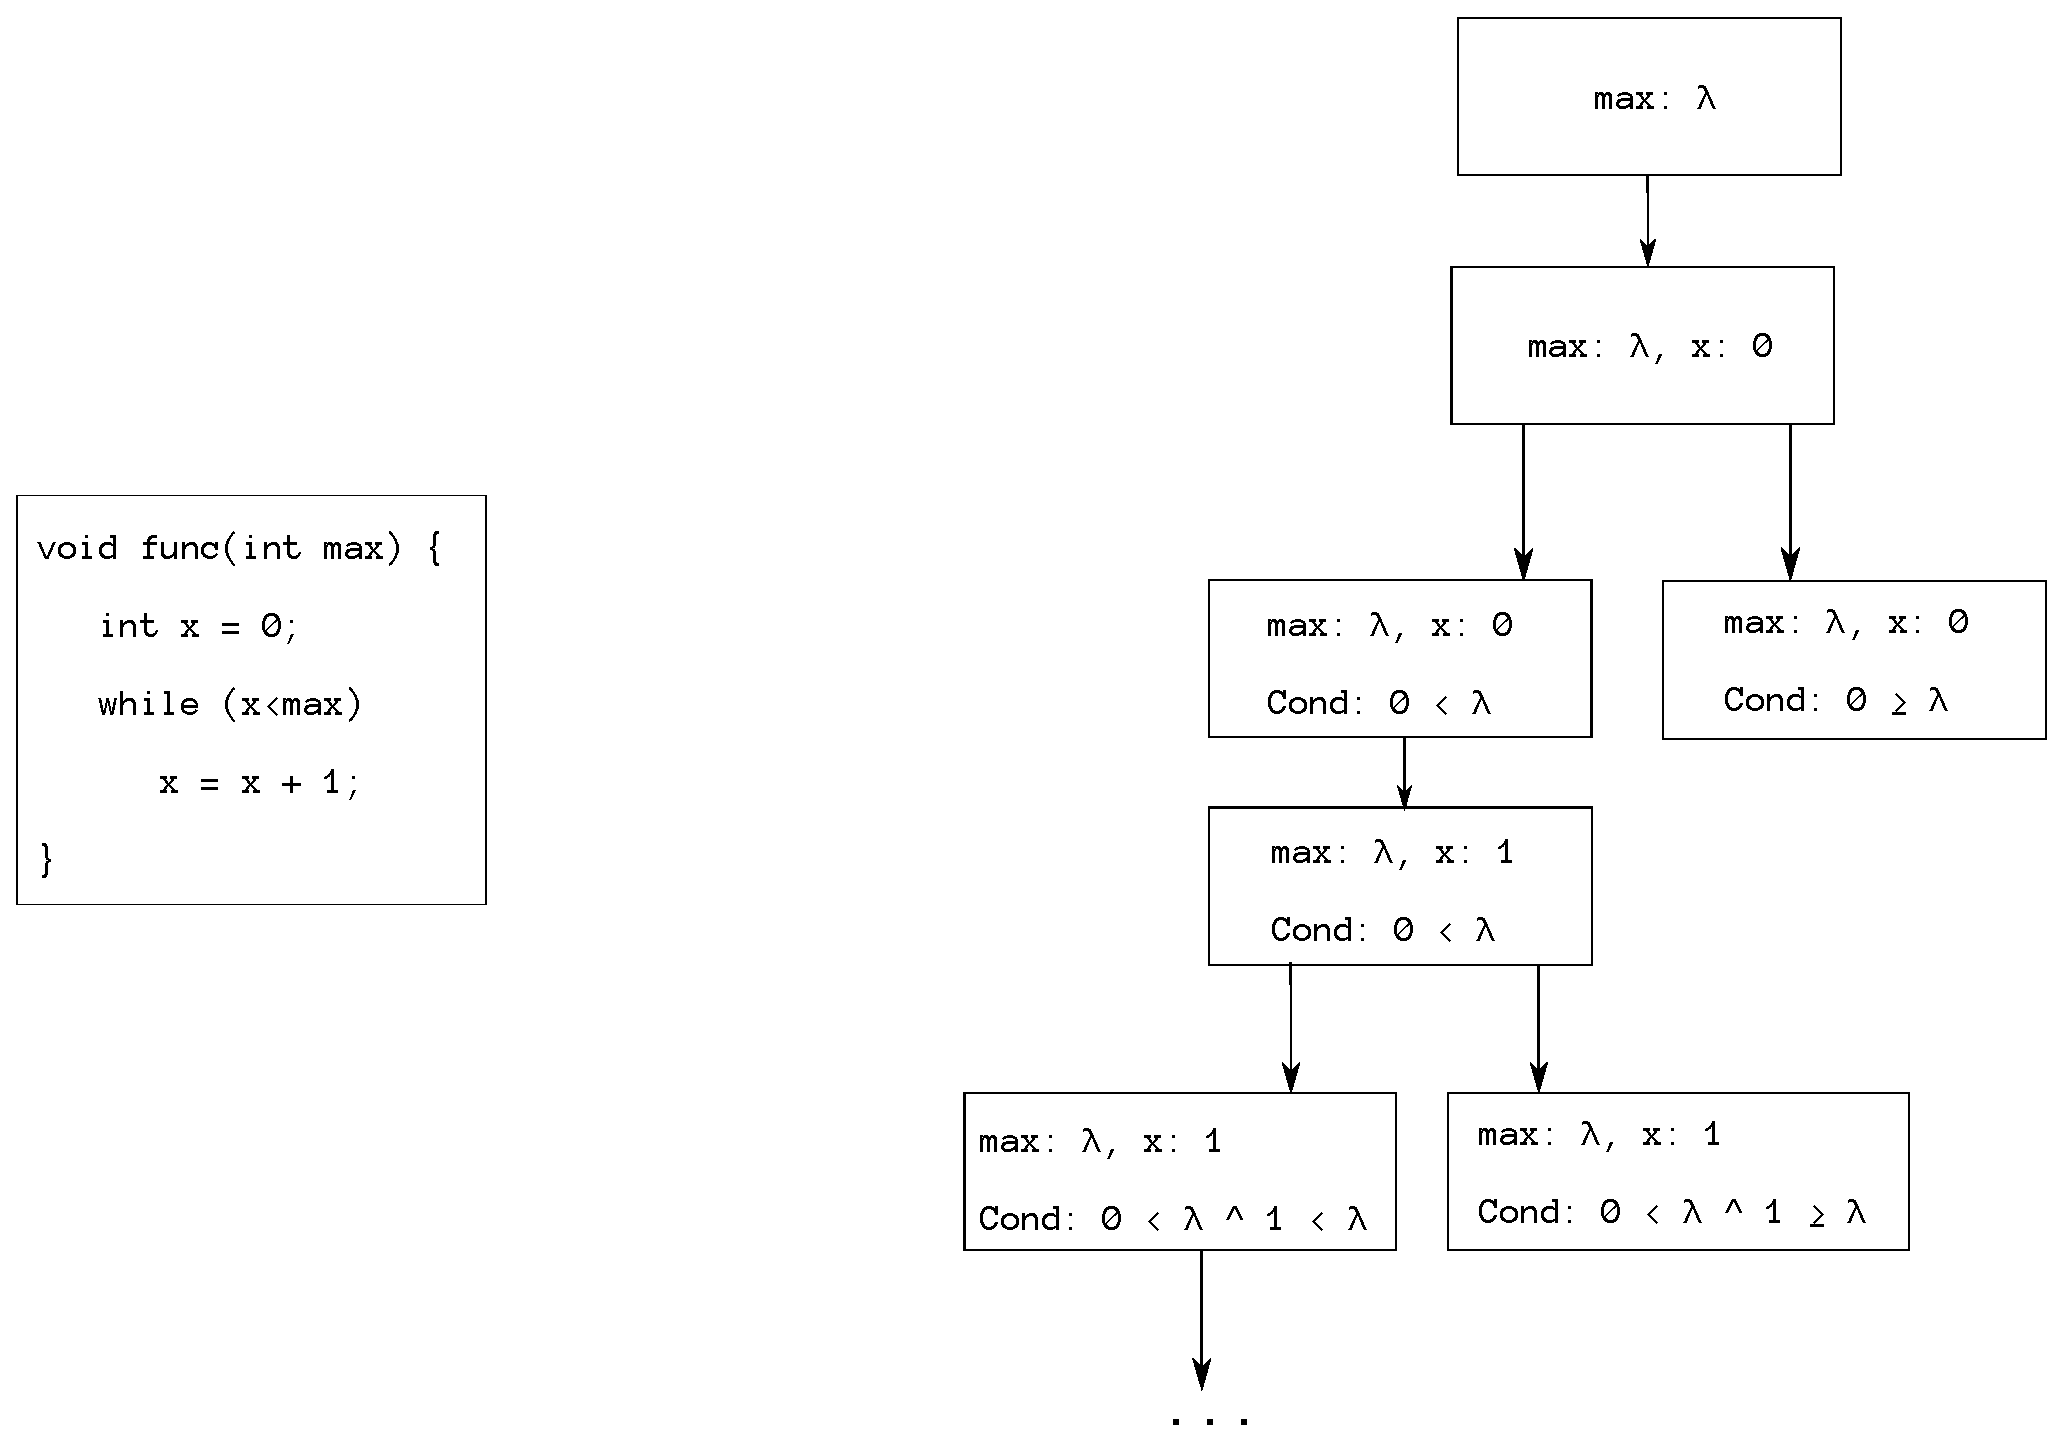
\includegraphics[width=0.8\textwidth]{figs/symbolicalle.eps}
    \caption{Example of a execution tree being constructed during symbolic execution for a sample code (variables being treated as a symbol  - symbol $\lambda$ in the Figure).}
    \label{fig:symbolic-execution}
\end{figure}


\subsubsection{Fuzzing}

Fuzzing can also be considered a specific form of an automated dynamic analysis. This technique consists of generating a massive amount of normal and abnormal inputs and feeding the target program with these generated inputs. Execution state is then monitored to identify if any of the inputs corrupted the execution flow. Fuzzing technique is easy to be deployed, with high accuracy as it is done in the real execution, and also easy to be scaled. However, fuzzing still has issues with low efficiency and code coverage, but as it is also a relatively new technique, a lot of research is being developed upon enhancing this technique, that has already become the state-of-art vulnerability discovery technique currently \cite{fuzzing}.


\subsection{Challenges in Vulnerability Discovery for IoT}

Regarding the vulnerability discovery methods presented in section \ref{subsec:vuln-disc}, these methods were developed to find vulnerabilities in general purpose computers such as home computers or servers. When trying to discover vulnerabilities in software developed for embedded hardware, researchers may face additional challenges~\cite{real-or-rehosted}.

The first challenge may be the acquisition of the target software. Many firmware images were only developed to work within their original hardware, and the only way to have a copy of the software may be opening the physical hardware and extracting the original system from one of its memories.

Another challenge is the dependency of the hardware. Firmware images are usually tied to the original hardware they were designed to operate with. To apply vulnerability discovery techniques in firmware files, we have to re-host the firmware so that it can be run inside an emulator and there we can apply the vulnerability discovery techniques. Usually, re-hosting is a process with a lot of challenges by its own~\cite{firmware-challenges}.

An additional challenge presented by firmware images that don't use a general purpose operating system (such as Linux, FreeRTOS, VxWorks) or firmware files that are really lean is that the vulnerability discovery methods aforementioned rely on monitoring operating system calls that indicate memory corruption. If the firmware don't implement security mechanisms that indicate memory corruption, it becomes a lot harder to automatically detect that the firmware execution reached an abnormal state (caused by the exploitation of an existent vulnerability) \cite{wycinwyc}.

\subsection{Tooling}

In this section, we will present the most common software tools used for firmware analysis and re-hosting. Most work produced relating to firmware analysis and re-hosting makes extensive use of the tools that will be mentioned here and therefore it is important to have an overall understanding about these tools.

\subsubsection{ {\tt binwalk} }

Binwalk \cite{github:binwalk} is a software with the purpose to identify and extract files from inside binary images. It was specifically developed to extract files and code embedded on firmware files, but it also became a popular tool for computer forensics and amongst players of computer security competitions (also known as Capture the Flag competitions). Binwalk achieves that by ``walking'' the binary image looking for magic numbers (file-type signatures). When a magic signature is found, then Binwalk has also the ability to try to extract the found file from inside the binary file. Table \ref{tab:magic-numbers} shows examples of file signatures (magic numbers) for common file-types.

\begin{table}[h]
\centering
\caption{Example of file-type signatures (magic numbers).}
\resizebox{\textwidth}{!}{\begin{tabular}{|c|c|c|}
\hline
\textbf{Hexadecimal Value}                                 & \textbf{ASCII Representation}                & \textbf{File-Type}                   \\ \hline
{\tt \footnotesize 89 50 4E 47 0D 0A 1A 0A}                & {\tt PNG}                     & Portable Network Graphics (PNG Image)\\
{\tt \footnotesize 4C 5A 49 50}                            & {\tt LZIP}                    & LZip Compressed File                 \\
{\tt \footnotesize 7F 45 4C 46}                            & {\tt ELF}                     & Linux Executable File (ELF)          \\
{\tt \footnotesize 25 50 44 46 2D}                         & {\tt \%PDF-}                  & PDF Document                         \\ \hline
\end{tabular}}
\label{tab:magic-numbers}
\end{table}


Binwalk is commonly used in most work related to firmware analysis, and it is usually the first tool used for firmware extraction. Binwalk also provides a Python application programming interface (API) that can be used to integrate Binwalk functionality inside a Python code.

In our work, a script originally developed for the Firmadyne \cite{firmadyne} making extensive use of the Binwalk API was slightly modified to extract the kernel and filesystem from the acquired firmware images.

Just out of curiosity, Binwalk was developed as an open source project in 2010. In 2017 the team behind Binwalk founded a company called ReFirm Labs and launched a commercial closed source version of the tool: Binwalk Enterprise. In early 2021, Microsoft acquired ReFirm Labs and is integrating the commercial version of the tool in it's Azure Defender for IoT product \cite{microsoft-refirmlabs}.

For our future research projects, our team inquired Microsoft about the Binwalk Enterprise pricing. The company was eager to make a cooperation and let our team participate in an early private preview of the Azure Defender for IoT product although we haven't used any of the mentioned commercial tools in this present work.

\begin{figure}[H]
    \centering
    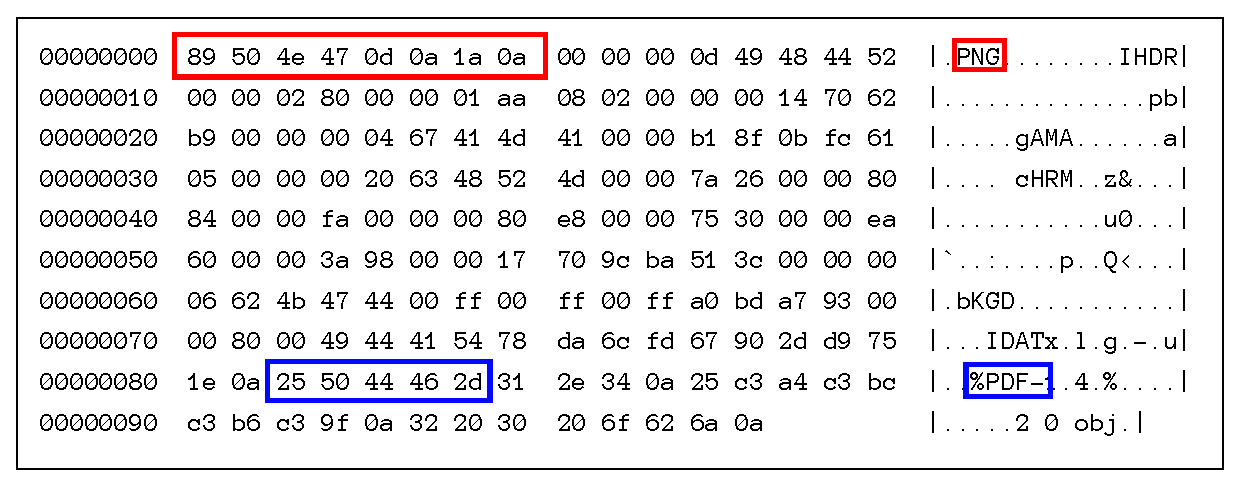
\includegraphics[width=0.7\textwidth]{figs/binwalk.eps}
    \caption{Example of magic numbers being found inside a binary file hexadecimal dump (commonly referred to as a file {\tt hexdump}). From this sample binary, Binwalk would be able to detect and possibly extract a Portable Network Graphics (PNG) image and a Portable Document Format (PDF) document.}
    \label{fig:binwalk}
\end{figure}


\subsubsection{ {\tt dd} }

The {\tt dd} software is part of the GNU Project and it is a command-line utility whose purpose is to convert and copy files for Unix-like operating systems. {\tt dd} is commonly used in firmware analysis for extracting files from a binary file. For most cases, Binwalk may be sufficient and most useful for identifying and extracting data from binary files. When Binwalk fails to extract a file (usually because the firmware is compressed in a way Binwalk can't recognize), {\tt dd} is a great tool to be used to perform the extraction manually.

\subsubsection{ {\tt QEMU} }
\label{sec:qemu}

QEMU \cite{qemu} is an open source machine emulator and virtualizer. It was designed to be a fast machine emulator and it works via binary translation. QEMU is capable of emulating several CPU architectures. As already mentioned in Section \ref{sec:rehosting}, QEMU can be used both in the ``user mode emulation'' to execute single binaries or in the ``system emulation'' mode, in which it can emulate a complete virtual machine.

In our work, as in most research we analysed, QEMU will be the main tool responsible for the re-hosting phase of our idealised architecture, in which it will ideally be used to emulate firmware execution outside it's original hardware, allowing us to dynamically analyse firmware execution and search for vulnerabilities.

\subsubsection{ {\tt Firmware-mod-kit} }

The {\tt Firmware-mod-kit} \cite{google-code:firmware-mod-kit} is actually a wrapper around the already mentioned {\tt dd} and Binwalk tools alongside other tools capable of extracting other types of filesystems that are not already contemplated by Binwalk. Although {\tt Firmware-mod-kit} was not used in our research project, it is not rare to see this tool in firmware analysis articles being used to extract and rebuild linux based firmware and because of that we decided it was worth mentioning it's existence. However, for more actual works, the tool is lacking recent support and we do not advise it usage.

\subsection{ Metasploit Framework }

The Metasploit Framework~\cite{github:metasploit} is an open-source tool designed to develop and execute exploits against a remote computer target. The Metasploit Framework holds a database of publicly disclosed and well known vulnerabilities for popular software, together with pre-configured exploit code that can be used to perform simple, low effort and automated attacks against vulnerable software.

The Metasploit Framework is not actually a common tool used when working with firmware, but it is a common tool used in security analysis. Some of the related work mention the Metasploit Framework tool, and we are also going to mention it furthermore in our work, so that's why we decided to also mention this tool in the tooling section.

\chapter{Related Work}\label{chap:related}
Considering the context of our study, to understand the running components (operating systems, file systems, services) in the router's firmware contributes to the re-hosting.  Re-hosting is a technique for executing a tightly coupled system in another hardware or platform (in our case, it means emulating the router firmware in a general purpose computer desktop).  Thus, our contribution relies upon this context.  We observed different approaches regarding overcoming re-hosting difficulties caused by the need for peripherals of the original hardware that are not present in the emulated device (the most challenging aspect of emulating a firmware). For example, the work of \cite{firmware-challenges} surveys the prominent techniques used in firmware re-hosting to bypass actual hardware dependency. Thereby, the four most common approaches are Partial Emulation, Fuzzing, Learning, and Abstraction Replacement. Also, a recent article discusses a novel approach that we will call here Symbolic Inference. We will briefly describe these approaches in the following sections.

\section{Partial Emulation}

Partial emulation, also known as ``hardware in the loop'', consists of emulating most firmware execution; however, redirecting to the actual device hardware calls when the firmware asks for a peripheral is infeasible. This approach requires having an actual device available, and for this reason, it does not scale. Execution fidelity, on the other hand, is pretty close to the actual hardware execution. The work of \cite{surrogates} enhances hardware redirecting by building a hardware bridge using an FPGA board to connect the PCI bus on the emulating host with the PCI bus on the actual embedded device, an approach they called {\tt SURROGATES}. Figure \ref{fig:surrogates} illustrates the approach used for the {\tt SURROGATES} solution.

\begin{figure}[H]
    \centering
    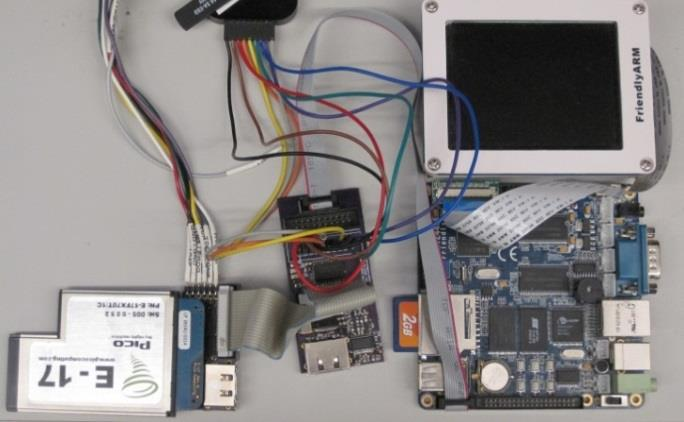
\includegraphics[width=0.7\textwidth]{figs/surrogates.png}
    \caption{FPGA gateway built to forward peripheral calls from the emulated system to the real device hardware. Developed as part of {\tt SURROGATES} solution \cite{surrogates}.}
    \label{fig:surrogates}
\end{figure}
The work of \cite{avatar2} extensively explores vulnerability discovery in embedded devices using the hardware in the loop technique. They use a symbolic engine builds upon QEMU called {\tt S2E} to search for vulnerabilities in IoT devices through re-hosting and to redirect peripherals calls to the actual hardware. In addition, they implement a tool called {\tt Avatar$^2$} as a reverse engineering framework based on the hardware in the loop approach.  Nonetheless, the dependency on the physical systems imposes barriers in testing and makes this alternative infeasible for our research.

\section{Fuzzing}

To overcome the partial emulating techniques, Fuzzing is a re-hosting approach to hardware dependence (not to be confused with fuzzing as a vulnerability discovery technique) because hardware calls to peripherals do not need the peripheral to be successful. Instead, the actual peripheral response request to the hardware call is just a binary value. Therefore, knowing the range of values that provide an acceptable answer to the hardware call, selecting any random value within this range is enough to keep executing the emulated system.

\cite{p2im} effectively implements this kind of hardware bypass.  The authors present an approach to model the interface between the processor and the peripheral. The method suggested is called {\tt P2IM} - Processor-Peripheral Interface Modeling.  However, it requires a human specialist to model the interface between the CPU and a specific peripheral to determine the specific range of values to each hardware call. Therefore, this approach also does not provide a scalable solution, requiring human intervention (to model the interface).

\section{Learning}

Learning is a similar approach to fuzzing for re-hosting, as it relies on the fact that to bypass hardware dependence, it is only needed to return expected values to hardware calls. However, the learning approach, as used in \cite{pretender} first monitors actual hardware execution and registers each hardware-peripheral interaction. Then it uses a Machine Learning algorithm to build a model of the interface (in contrast to using a human specialist as in the fuzzing approach). As a result, the learning technique produces a better interface to simulate peripheral interaction; however, it also depends on having the actual hardware first to build the interface's working model, which impedes its scalability and makes in an unsuitable solution for us.

\section{Abstraction Replacement}

Abstraction Replacement takes a different approach, and instead of producing answers to hardware calls that are similar to the responses real hardware would produce, this method tries to remove from the original firmware the hardware call, replacing it with another abstraction not requiring the actual hardware.

In the work of \cite{halucinator}, they develop the method called {\tt HALucinator}, whose idea is to search for Hardware Abstraction Layer (HAL) libraries inside the firmware and replace those libraries with custom libraries implemented by the researchers that do not require peripherals to work. However, this method still requires human intervention for each firmware and thus, still does not scale.

On the other hand, the work of \cite{firmadyne} implements a tool called {\tt Firmadyne}, whose approach to re-hosting consists of replacing the original kernel found on the firmware image with a custom implemented and instrumented kernel worked by their team (the same kernel is used to all firmware images emulated, regardless their original kernel version) together with applying some fixes to the filesystem (e.g replacing default root password and creating some essential directories). This approach allows firmware emulation to be done at scale, with the counterpart that the kernel replacement sacrifices emulation fidelity (because of the change in the kernel, emulation fidelity in in userspace at most). The authors of {\tt Firmadyne} also implemented a web scraper capable of downloading firmware binary from popular vendors website and then used {\tt Firmadyne} to emulate and perform security analysis on the downloaded firmware images.

Firmadyne architecture, shown on Figure \ref{fig:firmadyne}, is very much aligned with the architecture we first idealized for our research, and thus this tool will set the basis of the work presented in this paper. More details about Firmadyne architecture will be given in Chapter \ref{chap:screen}.

\begin{figure}[H]
    \centering
    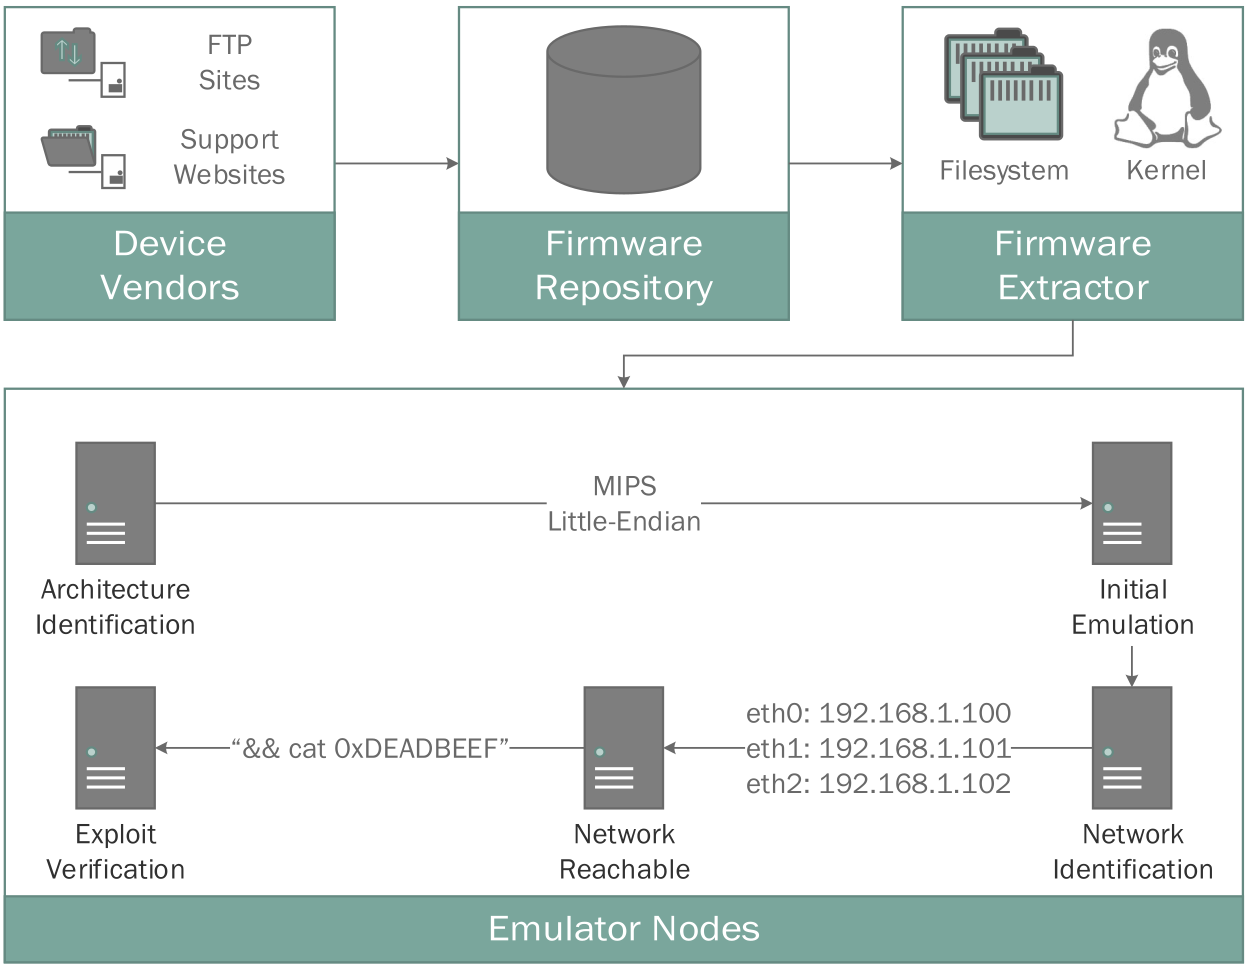
\includegraphics[width=0.6\textwidth]{figs/firmadyne.png}
    \caption{Firmadyne architecture~\cite{firmadyne}.}
    \label{fig:firmadyne}
\end{figure}

\section{Symbolic Inference}

A new approach to firmware emulation was proposed in the work of \cite{jetset}, in which the researchers hypothesize that the minimal behavior expected to boot a firmware to a point of interest by a security analyst could be inferred automatically. They then implemented a tool called Jetset that extends the idea of symbolic execution to model the hardware peripherals calls answers until firmware reaches a target address (e.g. boot finished). Their solution takes as inputs the executable code of the target, the memory layout of the target, the entry point address for execution start and the goal address that the analyst desires the code to reach.

The authors of Jetset then prove the capacities of their implemented tool by using it to perform the re-hosting of thirteen different pieces of firmware. The device in which Jetset was applied that resembles the most similarities with wireless routers is the Raspberry Pi 2 (based on the Bradcom BCM2836 System on a Chip [SoC] running on ARM architecture). For this device, the inputs needed for the proposed method to succeed are pieces of information extracted from the chip manufacturer documentation for the chip (datasheet). In terms of scalability, this is not ideal because one one need to gather information about the different SoC's of our targets, but the idea behind Jetset is very powerful and is a solution worth exploring.

\section{Summary}

% As we can see, many of the re-hosting techniques rely on non-scalable mechanisms. For example, Firmadyne provides an improvement to enable analysis at scale; however, it imposes limitations and remove much software running in kernel mode.  We present a proposal that differs from others by increasing the re-hosting coverage of operating systems in small and home-office systems (SOHO).  Our work provides a vision of operating systems to focus on, including a hardware architecture, version, and file systems.  Hence, identify dependencies in components (specific drivers) and maximize artifacts with favorable prominence (e.g., network stack).  As a result, it advances the state-of-the-art by bringing pieces of software left out of the emulation loop.

% ======== AQUI TEM MUDANÇA IMPORTANTE ========
As we can see, many of the re-hosting techniques rely on non-scalable mechanisms. For example, Firmadyne provides an improvement to enable analysis at scale; however, it imposes limitations and remove much software running in kernel mode. As in our work we are targeting a specific class of firmware, in this case wireless routers running on SOHO systems, we propose to make an adjustment in the approaches used for firmware re-hosting to use information gathered from freely available firmware images on the internet and use these pieces of information to enumerate firmware images features and components. This enumeration can be used to highlight prominent targets for security inspection and also to enhance the approach used for re-hosting. For instance, the kernel replacement done by Firmadyne could be done with a kernel more similar to the original kernel found on the firmware. 

In the next section, we will further discuss the approach that is going to be used in our research.

\chapter{SCREEN}\label{chap:screen}
% In this chapter, we will present the architecture our research proposes in order to evaluate the large-scale re-hosting of router firmware images and the innovative aspects of the approach intended in this project. Hence, we define SCREEN: {\bf S}craper, {\bf C}lustering, {\bf RE}-hosting, and {\bf E}xploitatio{\bf N}.

In this chapter, we will present the architecture our research proposes in order to evaluate the large-scale re-hosting of router firmware images and the innovative aspects of the approach intended in this project. This paper represents only part of the solution idealized for a bigger research project, to be conducted throughout the years by a team of researchers that have already been contributing to our efforts. Firmware analysis is a new subject for most of the team, and so the work described in the paper is just the starting point of our research, in which we familiarize ourselves with the field and explore the state-of-the-art related work. In this process, we already envisioned research opportunities and possible paths that can expand the state-of-the-art solutions in firmware re-hosting.

Our final goal with the complete research project is to evaluate the feasibility of a large-scale network attack targeting SOHO wireless routers. As mentioned in Chapter \ref{chap:introduction}, we will be taking an offensive security approach, in which we will incorporate the attackers' role in trying to find configuration flaws and security breaches in firmware images that are operating in wireless router devices in the real world. To achieve that, we will need to acquire router firmware images and conduct our research on top of the acquired data. 

Hence, we define SCREEN: {\bf S}craper, {\bf C}lustering, {\bf RE}-hosting, and {\bf E}xploitatio{\bf N}, the solution whose architecture will be described next.

\section{Complete Architecture Idealized}

This paper represents only part of the solution idealized for a bigger research project, to be conducted throughout the years by a team of researchers. Figure \ref{fig:architecture} illustrates the overview of the SCREEN architecture for the complete project, whereas in this paper we will focus on the re-hosting part (highlighted in the Figure) of the proposed architecture. 

As the re-hosting requires already acquired firmware data, a scraper is also going to be required for the research to start. Because of that, we will take advantage of an already implemented scraper (firmware acquisition is described in Section \ref{sec:firmware-aquisition}), but exploring its work or enhancing its capabilities will be out of the scope proposed for this work.

\begin{figure}[h]
    \centering
    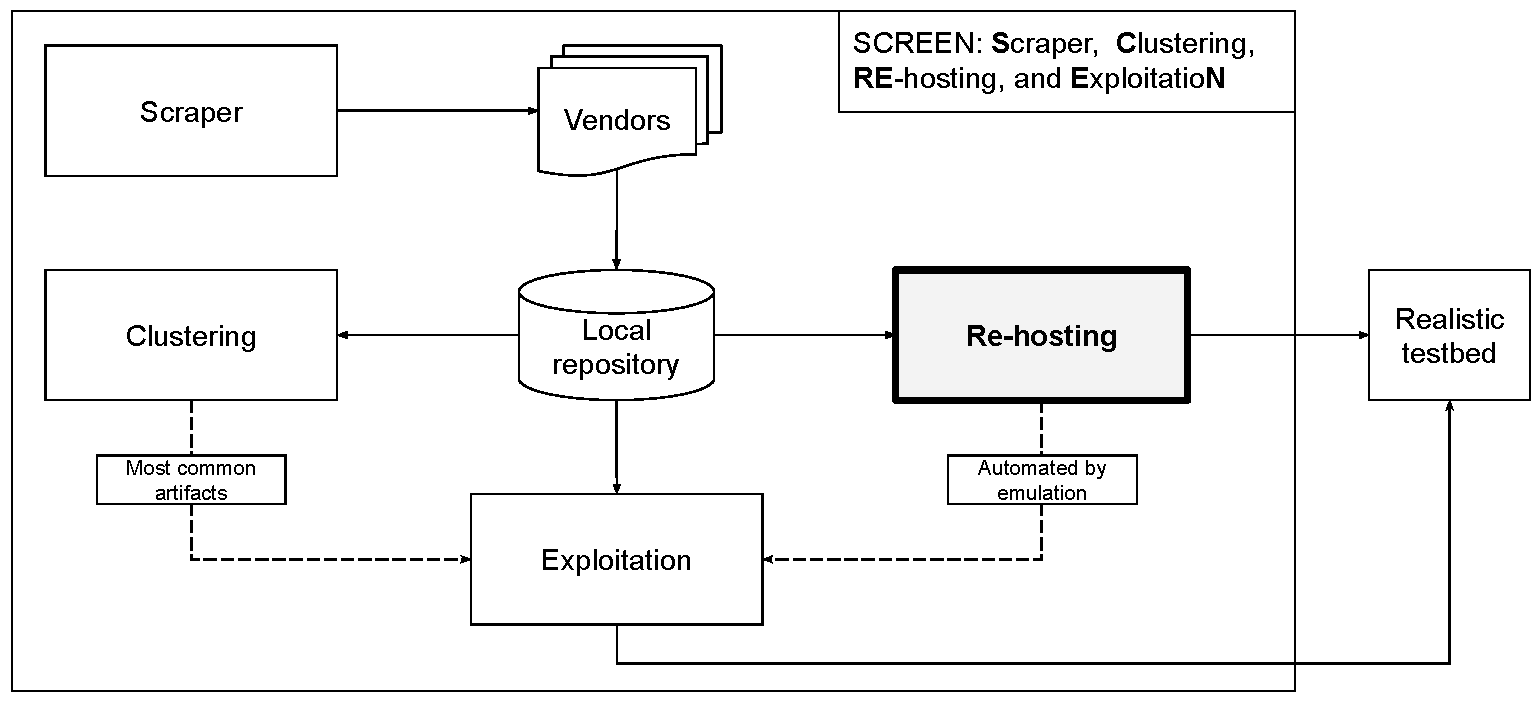
\includegraphics[width=0.85\textwidth]{figs/screen.pdf}
    \caption{Proposed architecture for SCREEN, our complete solution for firmware vulnerability analysis.}
    \label{fig:architecture}
\end{figure}


Considering the complete architecture illustrated by Figure \ref{fig:architecture}, everything starts with the scraper module (just mentioned) consisting of a web crawler responsible for entering router vendors' websites and downloading for a local repository (in our case to a simple directory) the biggest amount of firmware images available as possible. As mentioned, firmware images are a requirement for the re-hosting experiments to be conducted. So, in this stage, the scraper module is going to only serve the purpose of providing a minimum amount of firmware images to allow the research to proceed. Therefore, our approach will be to use a fork of the original Firmadyne's \cite{firmadyne} implemented scraper for now. In the future, if needed, our team is willing to update Firmadyne's scraper and also add more vendors to the list.

% From the local repository, two different modules will perform actions using the acquired firmware. The re-hosting module will be responsible for extracting firmware images (and collecting information about the firmware in the process) and preparing the firmware image to be emulated. As this module will be the focus of this research, section \ref{sec:re-hosting} will explain this process in detail. The other module to perform actions in firmware images contained in the local repository is the clustering module. This consists on searching for similarities and patterns amongst different firmware images, and collecting the most common artifacts present on the firmware images. The results obtained by the clustering modules can be used in further steps to improve the vulnerability analysis and discovery process.

From the local repository, two different modules will perform actions using the acquired firmware. The re-hosting module (the main subject of this work) will be responsible for extracting firmware images (and collecting information about the firmware in the process), enumerating firmware content, extracting statistics from the firmware repository and preparing the firmware image to be emulated. As this module will be the focus of this research, Sections \ref{sec:extraction} and \ref{sec:re-hosting} will explain this process in detail. For now, let us continue explaining the proposed architecture. 

% The other module to perform actions in firmware images contained in the local repository is the clustering module. This consists on searching for similarities and patterns amongst different firmware images, and collecting the most common artifacts present on the firmware images. The results obtained by the clustering modules can be used in further steps to improve the vulnerability analysis and discovery process.

The other module to perform actions in firmware images contained in the local repository is the clustering module. This consists of searching for similarities and patterns amongst different firmware images and collecting the most common artifacts present on the firmware images. The idea is to gather a lot of data in this process and try to apply state of art pattern discovery techniques. The plan is that the results obtained by the clustering module could be used in further steps to improve the vulnerability analysis and discovery process. For now, this module is only in the idealized architecture and this work does not contain any advances in implementing the clustering module. In fact, the clustering and exploitation modules are still subjects to be designed in further steps of the research to be conducted by our SCREEN contributors.

The final module of the architecture is the exploitation module, that as just mentioned is still only an idealization and open to changes. In this stage, the plan is to apply vulnerability analysis (using frameworks to detect known software vulnerabilities - such as the Metasploit framework) and vulnerability discovery (such as fuzzing techniques) on the emulated firmware to analyze its security performance.

In the next subsections we will describe more about how the extraction, enumeration, and re-hosting of the firmware files are going to be accomplished.

\section{Firmware Extraction}
\label{sec:extraction}

For the firmware extraction process, our research is going to focus on enhancing the original script provided with Firmadyne \cite{firmadyne} for firmware extraction developed in Python and making extensive use of {\tt binwalk}'s API. This original script uses {\tt binwalk} to recursively extract the firmware image setting a limit for depth and breadth in order to limit this process as it is very slow. To speed up the extraction, the {\tt /tmp} directory of the host system (which is used to temporarily store files during the firmware extraction process) is going to be mounted on the {\tt tmpfs} provided by the Linux kernel and that allow us to mount a directory in the Random Access Memory (RAM) instead of mounting it on the disk.

This can be done per session, using the {\tt mount} command, or an entry can be added to the {\tt /etc/fstab} file of the Linux system. The entries found in {\tt /etc/fstab} will be automatically mounted during the system boot process. For instance, for manually mounting a directory named {\tt /home/firm/extractdir} with 16GB of size into the {\tt tmpfs} (RAM) for a single session, command shown on Code \ref{code:tmpfs-manual} may be used (requires elevated privileges to run).

\begin{listing}[H]
\inputminted[breaklines]{text}{Code/tmpfs-mount}
\caption{Command-line to mount a directory into the TMPFS (RAM memory). Must be executed with root privileges.}
\label{code:tmpfs-manual}
\end{listing}

For automatically mounting the same directory into the {\tt tmpfs} during the boot process, with a size of 16 GB, the entry shown on Code \ref{code:tmpfs-fstab} should be added to the {\tt /etc/fstab} file:

\begin{listing}[H]
\inputminted[breaklines]{text}{Code/tmpfs-fstab}
\caption{Entry that needs to be added to the {\tt /etc/fstab} file in order to automatically mount a directory into the TMPFS during the boot process.}
\label{code:tmpfs-fstab}
\end{listing}

Nonetheless, this method of firmware extraction using the customized Firmadyne's \cite{firmadyne} extraction script is potentially incapable of automatically extracting some firmware images. Because not all firmware follows standard implementation, and frequently vendors obfuscate compression and file systems, we marked the failure subjects to posterior examination. Afterward, we inspect the marked ones to identify constraints and verify how to improve the automated image extraction. Then, subsequent modifying the extraction script, this entire process is repeated until satisfactory reach the maximum level in the extracted firmware images.

\section{Firmware Enumeration}

During the extraction phase, the extraction script, atop of Binwalk, tried to infer information about the kernel version within the firmware and the original architecture of the firmware in question. If these pieces of information are obtainable, they are stored within a database, associating the information with a firmware id (each firmware receives a unique identification number).

After a firmware filesystem is successfully extracted using the aforementioned extraction script, its content is then compressed and stored in a specific directory. Firmadyne already implements one tool that helps the task of enumerating firmware content. A Python script (named {\tt tar2db.py}) can be used to list the contents of a compressed filesystem for a given firmware image, and then the name of every file listed is stored in a database, associating the filename with the original firmware file.

Leveraging these mechanisms, we will explore how to automatically detect and extract data from within the firmware images together with a way to store and visualize this data.

\section{Re-hosting Process}
\label{sec:re-hosting}

We aim to maximize the portion of the original firmware during the re-hosting phase, absenting the original hardware. Firmadyne's approach to firmware re-hosting extracts from the original firmware image its original root filesystem and kernel. It then completely ignores the original kernel and replaces it with a custom instrumented kernel designed by the researchers (they developed one instrumented kernel for {\tt ARM} architecture and one for {\tt MIPS} architecture). Finally, the {\tt QEMU} tool is responsible for the emulation process, which uses binary translation to allow the execution of binaries from different architectures. The emulated firmware is emulated with {\tt QEMU} using the instrumented kernel together with the extracted filesystem from the original firmware.

Our approach to firmware re-hosting is similar to Firmadyne's one, with differences regarding the kernel replacement part. Instead of just building one heavily instrumented kernel and replacing all firmware images with that same instrumented kernel, we propose building-specific kernel versions on demand according to the original kernel used by the firmware image under emulation. With that, our heuristics correspond to use a more similar kernel to the original to reduce incompatibility with network drivers and modules and therefore increase the number of emulated firmware with a working network interface. In addition, increasing the emulation coverage allow us to extend the vulnerability analysis and discovery process to a more significant amount of router firmware images than the one covered by the original Firmadyne's implementation.

\subsection{Kernel Automated Compile}

This process of automated kernel cross-compilation, however, faces many issues. The first one is how to define a valid kernel compile configuration that results in a kernel that has the features expected in router firmware. Kernel compile configuration is a configuration file ({\tt .config}) where the user can configure an extensive list of parameters to include or exclude features to the compiled kernel.

These configuration files can be filled up by the user manually, via answering questions interactively in the command-line interface or ultimately adopting an existing file used by a current firmware's kernel previously compiled. Defining how to produce a good {\tt .config} file is already an open problem in our research. Another idea is to extract kernel compilation default configuration from OpenWrt Linux systems. The OpenWrt is a Linux targeted to serve as an open-firmware for wireless routers. Thereby, OpenWrt images may have kernel configurations compatible with most networking features expected from a wireless router. In this way, in this research, we plan to investigate the better way to produce a valid compilation configuration file to allow kernel compiling.

After choosing a valid kernel compilation configuration file, the kernel has to be cross-compiled in the host machine to compile for the architecture expected in the original firmware image. Unfortunately, kernel cross-compilation is also challenging, as the compilation process is heavily dependent on its toolchain (compiler, utilities, and libraries versions). Furthermore, it means that to compile multiple different kernel versions automatically; there must be a way to automatically switch between a set of known working toolchains for each kernel version.

Another approach, to reduce the number of parameters that need to be configured in order to build a very tailored kernel for each firmware, could be to use the enumeration and focus on building a repository with the most common kernel versions (or at least kernel families). Then, for the re-hosting, for each firmware image, a heuristic could be used to determine which compiled kernel from the repository is the most similar to the original kernel expected from the firmware. This matching kernel could then be selected to be used during the re-hosting process.

After compiling a kernel version that matches the original kernel, the firmware image is then ready to be emulated using the {\tt QEMU}. First, the newly compiled kernel serves as firmware in emulation with the original filesystem extracted from the firmware sample. After that, following the work of \cite{firmadyne}, we evaluate if these emulated firmware images can infer and configure the network successfully. If that is the case, vulnerability analysis and discovery techniques are applied (using standard tools for this purpose). Finally, the results obtained are helpful to evaluate overall firmware security, reporting the mapped vulnerable products (if that happens) to the vendor.

Figure \ref{fig:firmadyne-screen-compare} illustrates how the SCREEN approach to re-hosting differs from the one used by Firmadyne. While Firmadyne uses one heavily instrumented kernel with all firmware images during the re-hosting process, SCREEN will build kernels using the information gathered from the firmware images and select a more suitable kernel from the repository to use when re-hosting a specific firmware image.

\begin{figure}[h]
     \centering
     \begin{subfigure}[b]{0.45\textwidth}
         \centering
         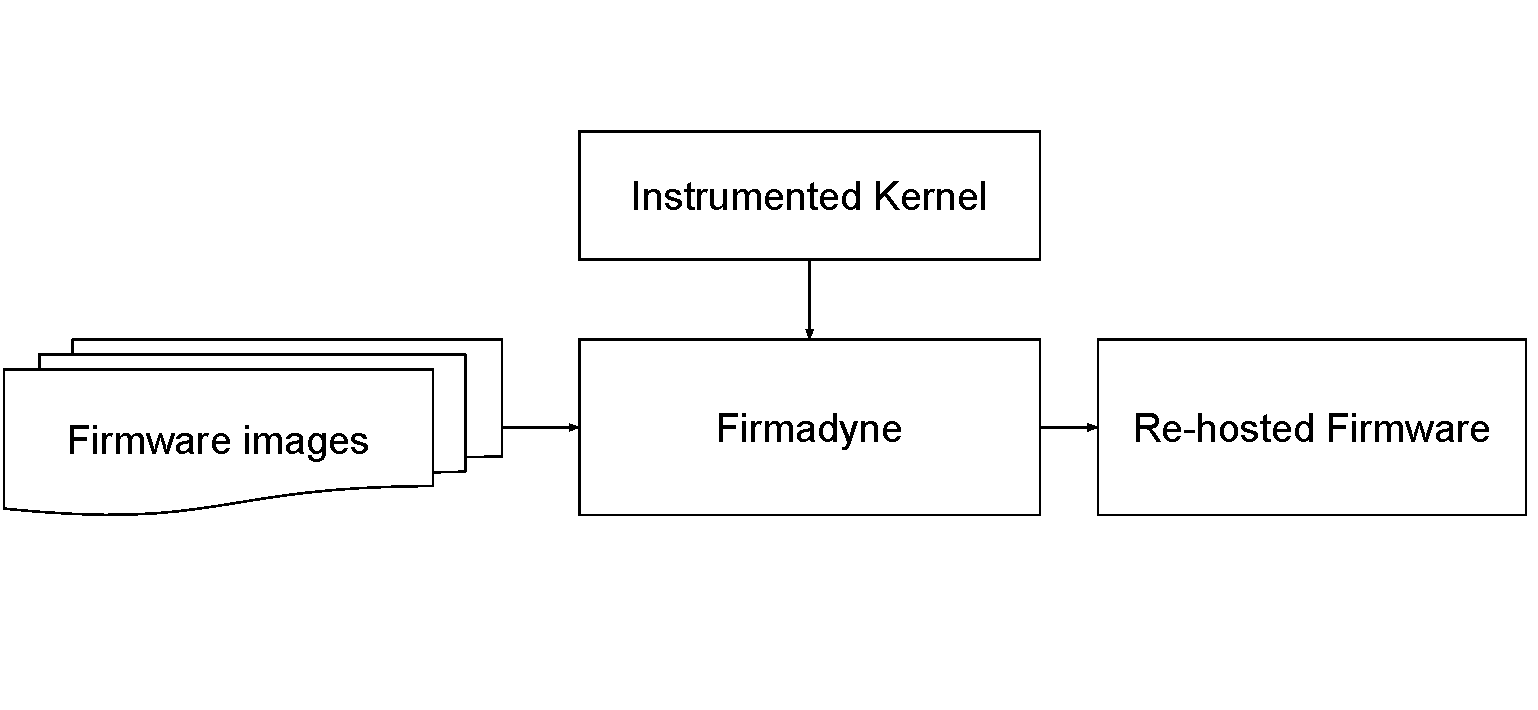
\includegraphics[width=\textwidth]{figs/Firmadyne-Approach.pdf}
         \caption{Firmadyne approach to re-hosting.}
         \label{fig:firmadyne-approach}
     \end{subfigure}
     \hfill
     \begin{subfigure}[b]{0.45\textwidth}
         \centering
         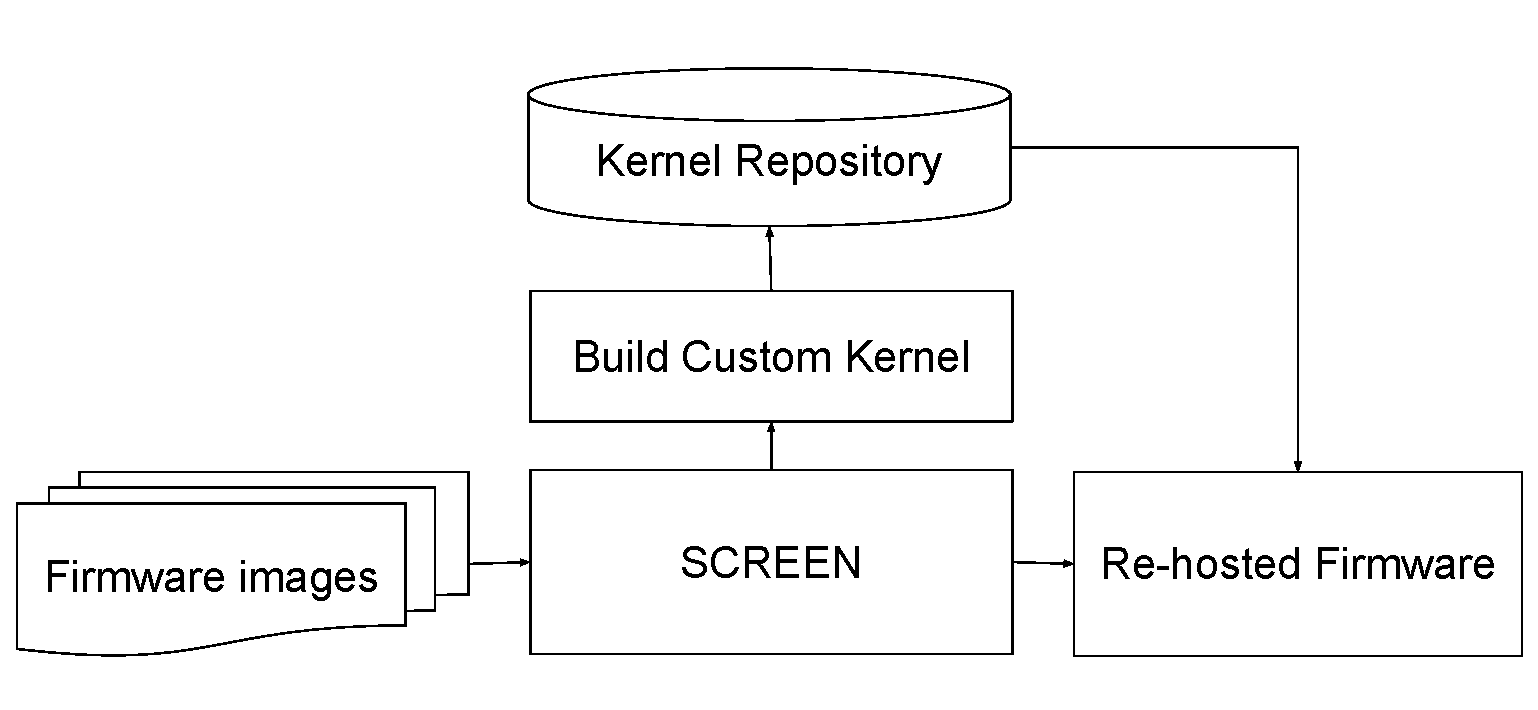
\includegraphics[width=\textwidth]{figs/SCREEN-Approach.pdf}
         \caption{SCREEN approach to re-hosting.}
         \label{fig:screen-approach}
     \end{subfigure}
        \caption{Comparison between the approaches used by Firmadyne and SCREEN during the re-hosting phase.}
        \label{fig:firmadyne-screen-compare}
\end{figure}

\subsection{Re-hosting execution}

We will also explore how to manually perform a firmware re-hosting by using {\tt QEMU} to start a system mode emulation with a minimal filesystem and kernel and then copy to this minimal system the essential files and configuration responsible for executing the basic behavior expected from the firmware. This will be done as a way to gain a deeper understanding of how to use the {\tt QEMU} emulator and to gain knowledge about the practical aspects of emulating firmware.

After that, we will explore how to perform re-hosting using other research products such as Firmadyne~\cite{firmadyne} and Jetset~\cite{jetset} with a critical view on how these solutions could be modified to enhance the re-hosting phase and increase the number of successfully re-hosted firmware, as this would allow us to (in further research projects) to perform security analysis on a larger number of firmware images.

\chapter{Experiments \& Results}\label{chap:exp_and_results}
In this chapter we will describe the work that has been done to perform the firmware acquisition, extraction and enumeration together with the statistics that we were able to extract from the results obtained. We will also describe the results we had when investigating and experimenting with kernel compilation and firmware emulation using both a manual approach and an automated approach via Firmadyne~\cite{firmadyne}.

\section{Work Environment}

Before discussing our results, this section will explain how our team has set up our software work environment. A personal computer was designated to work as a server. This server was then configured with a virtualization solution called Proxmox Virtual Environment\footnote{\url{https://www.proxmox.com/en/proxmox-ve}} as its operating system. Proxmox VE is a Linux operating system (based on the Debian distribution) that acts as a virtualization server. It provides a web interface in which the user can create and manage virtual machines. Proxmox VE uses the already mentioned QEMU \cite{qemu} (mentioned in Sections \ref{sec:re-hosting} and \ref{sec:qemu}) and the Linux KVM technology as a backend, and provides a hypervisor for managing containers and virtual machines.

This setup allows us to easily create virtual machines to test software in an environment of isolation, save virtual machines disk snapshots and roll back in time if needed. A main guest virtual machine with Debian 10 was selected to host our main efforts. Table \ref{tab:vm-specs} shows the specifications of the machines (host and virtual machine) used as our main work environment. The access to the machines was done using the Secure Shell (SSH) protocol.

\begin{table}[H]
\centering
\caption{Specifications for the host machine and main virtual machine used in our project.}
\begin{tabular}{|c|c|c|}
\hline
\textbf{Specifications} & \textbf{Host} & \textbf{Guest VM} \\ \hline
Operating System        & Proxmox VE           & Debian 10             \\
Kernel Version          & {\tt5.4.128-1-pve}   & {\tt 4.19.0-18-amd64} \\
CPU Model               & AMD Ryzen 5 2600     & {\tt kvm64}           \\
Number of Cores         & 6 Cores              & 4 Cores               \\
Number of Threads       & 12 Threads           & 4 Threads             \\
Memory                  & 32 GB                & 20 GB                 \\ \hline
\end{tabular}
\label{tab:vm-specs}
\end{table}

Furthermore, to enhance the experience when working connected to a remote machine using the SSH protocol, some tools were extensively used in our work. Just for the record, we will list here some of the utilities we used as this can help other people that work in similar environments, in which remote work via SSH protocol is a routine.

\begin{itemize}
    \item \textbf{Tmux}: Utility to save SSH sessions. Using Tmux one can create a session inside the remote server. Sessions can be attached and detached, in a way that a person can leave processes running in a remote machine and then close the terminal running the SSH client, in a way that the running process will keep running inside the remote machine. Afterward, the user can simply join the remote Tmux session again and he will be reattached to the running processes he left in the previous session.
    
    \item {\tt ngrok}: This tool provides a way to easily open network tunnels to expose a service on the internet without requiring the user to forward ports in the network router to expose services in its local network. The user can choose which protocol and port {\tt ngrok} will expose to the internet, and the tool will provide a Uniform Resource Locator (URL) that forwards internet connection to the local service the user has exposed. A daemon running {\tt ngrok} was configured in our guest Virtual Machine (VM) allowing us to work on our server anywhere on the internet (outside our local area network [LAN]).
\end{itemize}

It's also worth mentioning that we also used the PostgreSQL database to save interesting data. Interaction with the database was done using the {\tt psql} command-line tool. PostgreSQL was already a requirement for the Firmadyne~\cite{firmadyne} tool. Hence, we decided to alter the schema that was already being used to add more columns in order to hold data we decided to gather from the firmware images.

\section{Jupyter Notebooks}

In order to organize work, especially as we intend to collaborate both as a team and also with external researchers, during our experiments, we felt the need to have a tool to help us record the experiments and to save the acquired information during the experimentation phase. Therefore, we decided a good fit for this need was to use Jupyter Notebooks as a way to report experiments and results. Jupyter Notebooks are a way to save documents containing formatted text (in Markdown language) with snippets of code (in Python or shell scripts) and its respective outputs.

Notebooks containing the code that was executed in order to extract information from the firmware images and to produce the results shown on this paper can be found on this project repository \cite{github:c2dc-toso} together with the output produced by their execution. Figure \ref{fig:jupyter} shows the interface of one of the implemented Jupyter notebooks.

\begin{figure}[H]
    \centering
    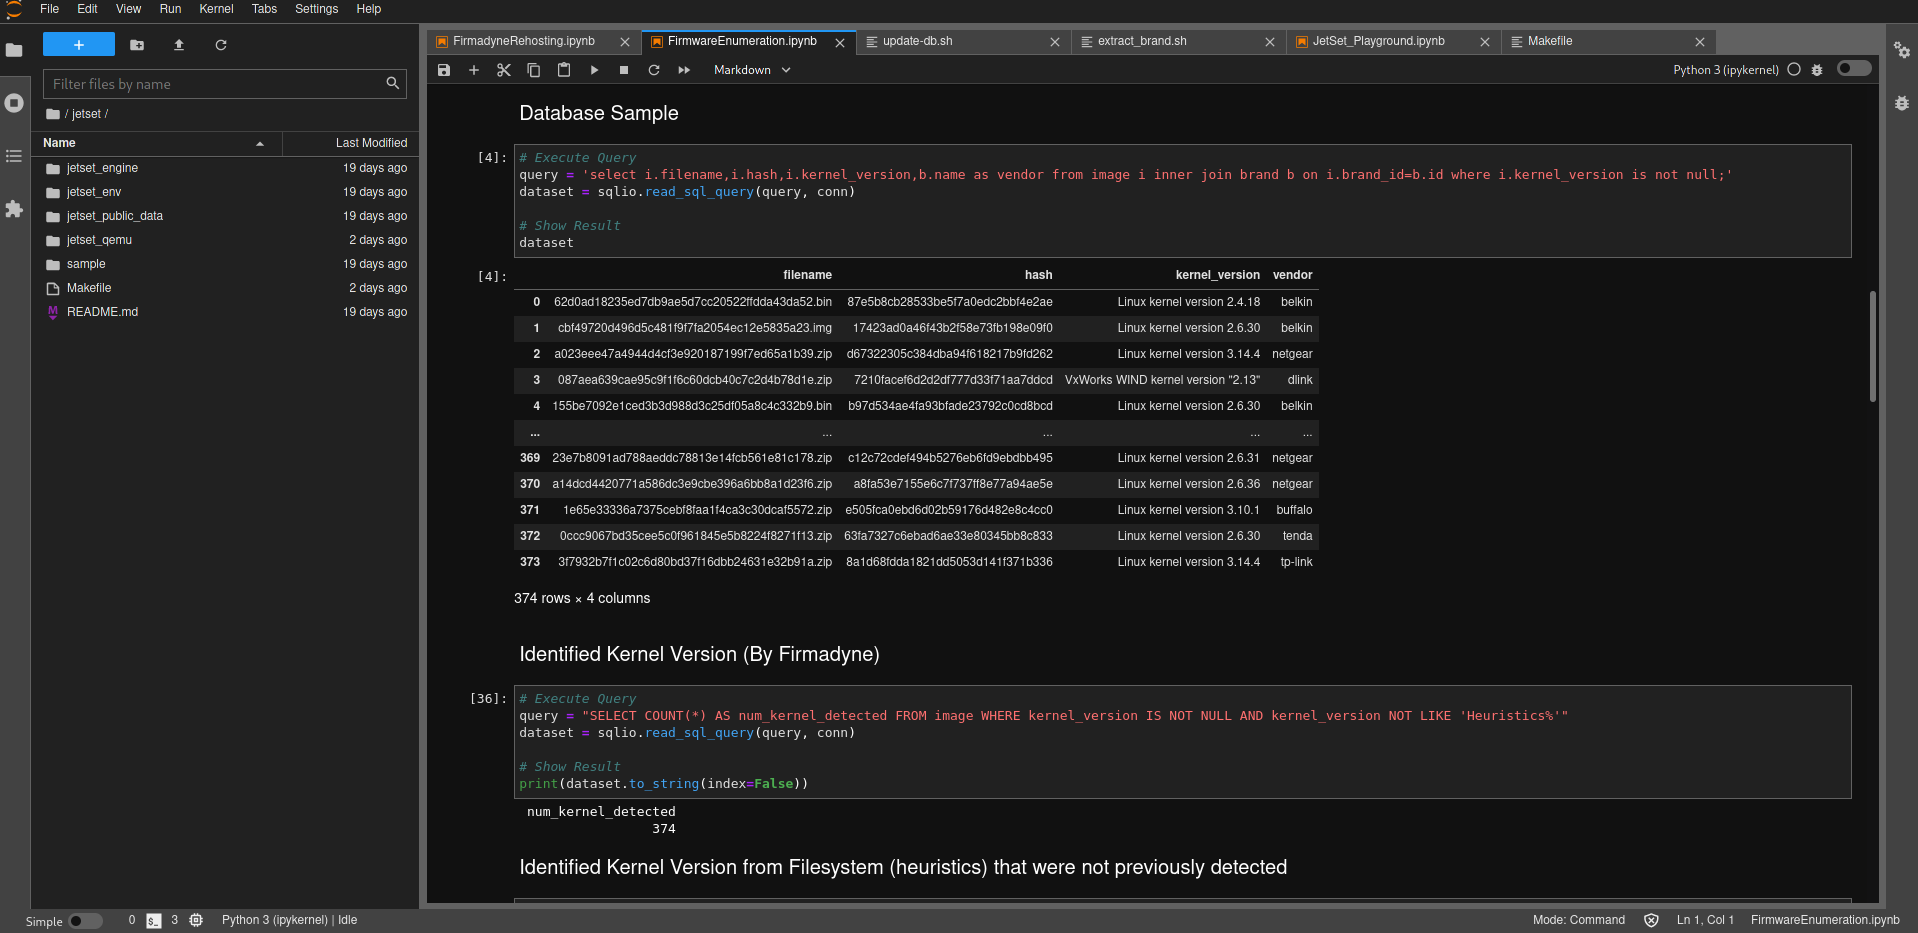
\includegraphics[width=1.0\textwidth]{figs/jupyter.png}
    \caption{Jupyter Notebook interface (showing firmware enumeration notebook).}
    \label{fig:jupyter}
\end{figure}

\section{Firmware acquisition}
\label{sec:firmware-aquisition}

For the firmware acquisition, we used a fork of the Firmadyne's \cite{firmadyne} original scraper \cite{github:scraper}. This modified scraper version has fixed some compatibility issues the original scraper has with Python 3 and also updates the spiders to match the more updated versions of vendors' websites. Without modifying any of the spiders provided by the scraper, we executed it to automatically find and download firmware from all the possible vendors implemented, which by default means 11 wireless router firmware manufacturers and 3 open-source firmware projects (OpenWrt, Tomato and pfSense).

As the project is part of a team research, and to facilitate the research setup between different machines, we also implemented a script to automate the execution of the scraper and to enumerate the scraped firmware images for each vendor. This implemented automation proved useful when we wanted to set up a new machine to work on our project.

In total, 9176 firmware images were downloaded throughout this process. Table \ref{tab:scraper}shows the number of firmware images and their combined file size for each vendor.

\begin{table}[H]
\centering
\caption{Downloaded firmware images per vendor. Vendors marked with $^*$ refer to open source projects.}
\begin{tabular}{|c|c|c|}
\hline
\textbf{Vendor} & \textbf{Firmware Images} & \textbf{Combined File Size} \\ \hline
OpenWrt$^*$     & 3898                     & 15 GB                       \\ 
Netgear         & 1544                     & 48 GB                       \\ 
MikroTik        & 873                      & 11 GB                       \\ 
TP-Link         & 788                      & 7.2 GB                      \\ 
D-Link          & 591                      & 8.8 GB                      \\ 
Polycom         & 547                      & 136 GB                      \\ 
Tomato (Shibby)$^*$ & 321                      & 2.3 GB                      \\ 
QNAP            & 279                      & 43 GB                       \\ 
Tenda           & 176                      & 825 MB                      \\ 
Ubiquiti        & 78                       & 2.3 GB                      \\ 
Belkin          & 36                       & 267 M                       \\ 
Mercury         & 33                       & 25 MB                       \\ 
pfSense$^*$     & 6                        & 2.2 GB                      \\ 
Buffalo         & 6                        & 75 MB                       \\ \hline

\end{tabular}
\label{tab:scraper}
\end{table}

% Note that the scraper also download firmware images from the OpenWrt project, which aims to develop a highly extensible GNU/Linux distribution suited for embedded devices (specially wireless routers). Because OpenWrt is not really a wireless router manufacturer, in the next statistics regarding the firmware images, the OpenWrt will be considered apart.

Note that the scraper also downloads firmware images from some open-source firmware projects, such as the OpenWrt project, which aims to develop a highly extensible GNU/Linux distribution suited for embedded devices (especially wireless routers). Because these open source projects are not really wireless router manufacturers, in the next statistics regarding the firmware images, statistics with and without these projects will be given.

As the goal of this work is towards the process of re-hosting, this amount of firmware images is already enough for initial experiments with automated re-hosting. In further work, more vendors' pages can be crawled, and we can update scraper's spiders if we judge there is a need for a larger volume of firmware images. Also, just for the record, one of our contributors has already implemented a spider to acquire firmware from a vendor that is not contemplated on the original scraper list (firmware from the ASUS manufacturer), but this implemented spider was posterior to our data acquisition and thus it was not used for the results in this paper.

\section{Firmadyne Automation}

Although Firmadyne~\cite{firmadyne} has already implemented code to perform firmware acquisition (with the scraper), extraction and re-hosting, there is no code that integrates and automated these actions - at least in the code provided by Firmadyne's public GitHub repository\footnote{\url{https://github.com/firmadyne/firmadyne}}. In this sense, we implemented a lot of shell scripts to automate the execution of Firmadyne's atomic actions. More than that, in our Jupyter notebooks, we show code to automate steps from Firmadyne execution and to programmatically extract important data and statistics from the firmware directory and Firmadyne's original database.

Also, as Firmadyne is only the product of a research project, and not a commercial software or community-backed open-source project, there is not extensive documentation around the tool, so to better understand what the software is doing and to learn how to use it properly, there was a lot of ``reverse engineering'' (code reading and following the execution flow) involved in this process. Actually, some parts of the original code were even adapted to better suit our needs.

\section{Firmware extraction}
\label{sec:firmware-extraction}

Firmware extraction was heavily based on the usage of the {\tt binwalk} tool, whose usage was wrapped inside a script provided by Firmadyne \cite{firmadyne}. This script, when executed with a firmware image as a parameter, recursively tries to extract files using {\tt binwalk} for this purpose. It defines a breadth and depth limit to this recursion strategy. During the extraction process, the script then tries to identify if any of the extracted directories has a Linux root directory structure (i.e. has {\tt /bin}, {\tt /etc}, {\tt /usr} directories and so on). If that is the case, then this filesystem structure is compressed and stored in a separate location (also defined as a parameter to the script). 21.48\% of the total amount of firmware files (1971 from 9176 images) were successfully extracted by Firmadyne's \cite{firmadyne} extraction script. Of these extracted images, 97.21\% (1916 images) had the root filesystem extracted and of these, 94.89\% (1818 images) had the architecture identified. Architecture identification is done by reading files in filesystem directories that should contain binary files (e.g. {\tt /bin} or {\tt /sbin}) and reading the header of these files (and comparing with the binary header expected for an executable file in any architecture).

Kernel detection is done by reading each entry identified by {\tt binwalk} in the extraction process and detecting known kernel types. These are also extracted and stored in a separate location. When using the script, the user has the option to disable kernel extraction, as this greatly improves execution speed since {\tt binwalk} spends a lot of effort in the extraction process. If kernel extraction is not disabled by the user, then the script also tries to identify kernel version and store this information in Firmadyne's \cite{firmadyne} database if found.

When extracting firmware, if Firmadyne's extraction script is capable of identifying the original firmware filesystem, its structure (only the names of each file) is saved into a database, associating each of the filenames with the firmware image identification number (image ID). After that, the original filesystem (with files contents) is compressed and saved in an output folder. Therefore, it is easy to search for files inside the extracted firmware images as one can easily query the database to search for a specific filename. If the content of a file is desired, the associated compressed filesystem can be extracted to recover the desired file content. Figure \ref{fig:sql-schema} illustrates with a few columns how the database is structured (only part of the schema and the data is shown on the image). The {\tt object\_to\_image} table from the database can be queried to search for specific files inside the compressed filesystem of the firmware images.

\begin{figure}[H]
    \centering
    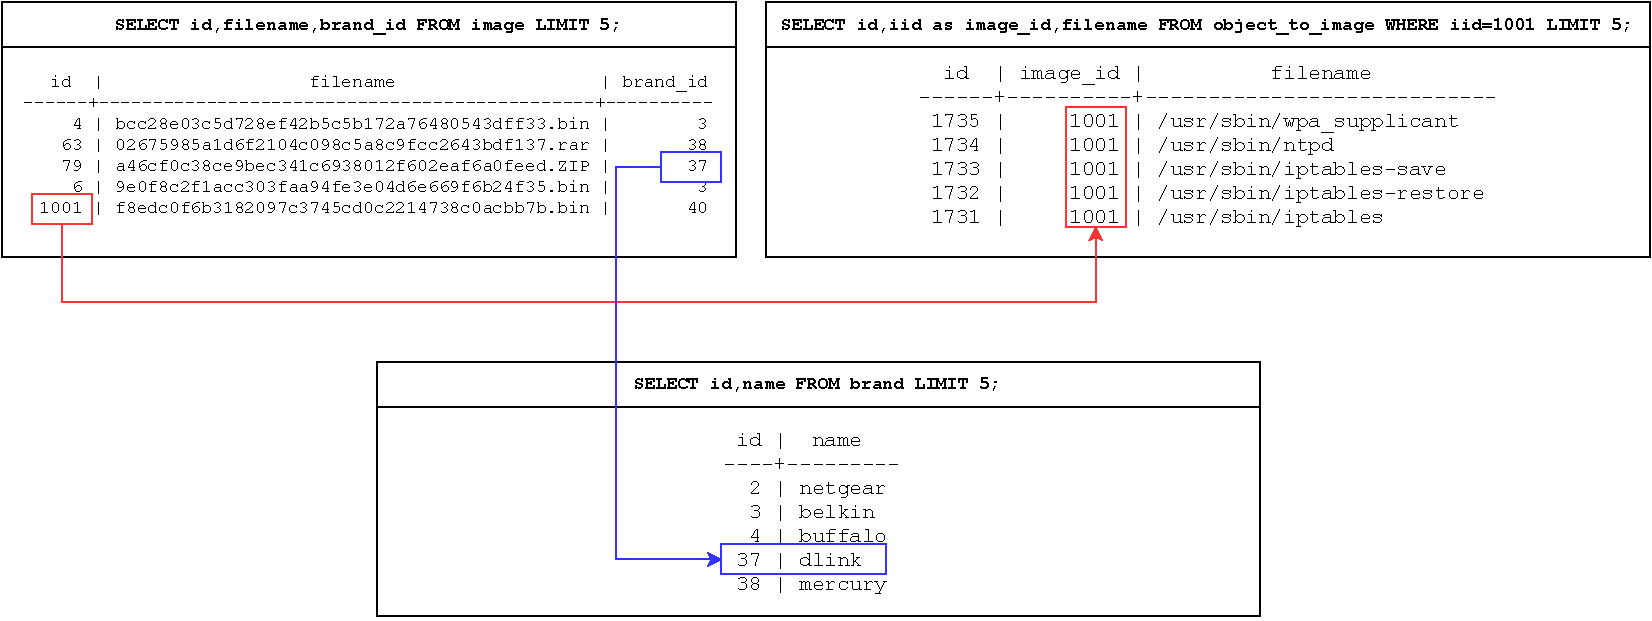
\includegraphics[width=1.0 \textwidth]{figs/SQL_Schema.pdf}
    \caption{Part of the database structure showing the relation between some tables. Note that the whole database contains more tables, columns and data.}
    \label{fig:sql-schema}
\end{figure}

As not all kernels are identified by the {\tt binwalk} tool during the extraction phase, we also developed a heuristic that uses regular expressions to search the extracted filesystem of each firmware image (querying the database) whose kernel was not identified during extraction and try to find directories that could reveal kernel version (e.g. {\tt /lib/modules/2.6.31} is an indication that this image contains a 2.6.31 Linux kernel). This search is extremely fast compared to the filesystem extraction process and increased the number of kernel versions detected. Initially, with Firmadyne's \cite{firmadyne} original extraction script, only 374 kernels were identified amongst the 1971 (18.98\%) of the total amount of firmware images. After running the described heuristics to determine kernel version from the filesystem, the number of identified kernels increased to 1812 (384.49\% greater).

When considering only the firmware files with root filesystem extracted and architecture identified, 97.85\% (1779 images) had the kernel identified. That is, 1779 firmware images of our dataset had its complete tuple identification: Architecture, Kernel Version and Root Filesystem. Figure \ref{fig:stats-funnel} shows the funnel of success for firmware extraction and illustrates the statistics just described.

\begin{figure}[H]
    \centering
    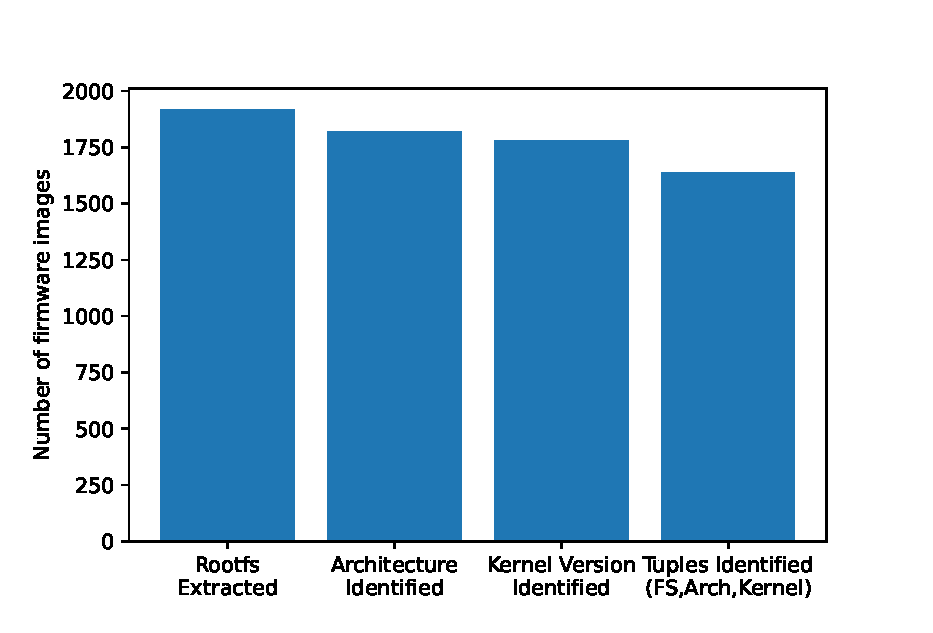
\includegraphics[width=0.90\textwidth]{figs/extraction_funnel.eps}
    \caption{Success funnel for firmware image extraction.}
    \label{fig:stats-funnel}
\end{figure}


It was also identified two issues in the extraction process. Some kernel image media types (also known as Multipurpose Internet Mail Extension [MIME] types) were incorrectly identified as a type that was on the extraction script blacklist. This could be easily corrected by excluding the identified type from the blacklist. The second issue is related to the recursive extraction process. The limits in breadth and depth exploration allow the {\tt binwalk} tool to have usable performance, but in some cases these limits were in fact responsible for the firmware extraction to be unsuccessful. Therefore, we believe that using a heuristic to select files with the most potential to hold firmware kernel or filesystem to be extracted next. This way we can still have breadth and depth limits to maintain the extraction process feasible but it would also focus the extraction in files that are more prominent. This approach of using heuristics although idealized was not yet implemented in our work.

Another enhancement we developed to the extraction process was the ability to extract additional kernel information. During kernel extraction, the kernel binary file is scanned for American Standard Code for Information Interchange (ASCII) strings and from the result of this search we then extract kernel banner (a string containing kernel version, compiler version used during kernel compilation, compilation date and email of the developer who compiled the kernel) or identify for instance if the system being extracted refers to an OpenWrt Linux (even if the firmware manufacturer is not OpenWrt). These additional pieces of information are also stored in Firmadyne's \cite{firmadyne} database, which had its schema altered to contain a new column to store the extra information for a given firmware image.

% Falar das estatísticas; Colocar tabela com as estatísticas

\subsection{Architecture and Kernel Statistics}

Regarding firmware extraction and feature identification, we collected some statistics that may help the following steps of this work in kernel compilation and firmware re-hosting. Table \ref{tab:arch-stats} shows the number of firmware images detected for each architecture identified when not considering the OpenWrt acquired firmware images. Also Tables \ref{tab:kernel-stats} and \ref{tab:kernel-family-stats} shows the five most common kernel versions and kernel families respectively when not considering OpenWrt, Tomato (Shibby) and pfSense. Finally, Tables \ref{tab:arch-stats-openwrt}, \ref{tab:kernel-stats-openwrt} and \ref{tab:kernel-family-stats-openwrt} shows the architecture, kernel version and kernel family statistics when also considering the OpenWrt, Tomato (Shibby) and pfSense firmware images.

The decision to include statistics with and without the aforementioned vendors' firmware images takes into consideration the fact that the three names represent open projects and they may not represent firmware statistics that are aligned with the firmware in commercial products. For instance, OpenWrt is a project led by the community to develop a GNU/Linux firmware that could easily be extended by developers and act as a framework for developing applications for embedded devices. In the project's official documentation it is stated that ``\textit{In practice, this means that you can have all the features you need with none of the bloat, powered by a Linux kernel that's more recent than most other distributions.}'', which means that by design OpenWrt kernel version statistics might not be befitting other vendor's statistics.

\begin{table}[H]
\centering
\caption{Number of images identified for each found architecture without considering OpenWrt, Tomato and pfSense firmware images.}
\begin{tabular}{|c|c|}
\hline
\textbf{Architecture}       & \textbf{Quantity of Images} \\ \hline
{\tt mipseb}                &  300                        \\ 
{\tt mipsel}                &  197                        \\ 
{\tt armel}                 &  182                        \\ 
{\tt ppceb}                 &   83                        \\ 
{\tt intelel}               &   69                        \\ 
{\tt intel64el}             &    4                        \\ 
{\tt mips64eb}              &    4                        \\ \hline
\end{tabular}
\label{tab:arch-stats}
\end{table}

\begin{table}[H]
\centering
\caption{Five most common kernel versions found in extracted firmware images without considering OpenWrt, Tomato and pfSense firmware images.}
\begin{tabular}{|c|c|}
\hline
\textbf{Kernel Version} & \textbf{Quantity of Images} \\ \hline
3.3.5                  & 546                 \\ 
2.6.36                 &  59                 \\ 
2.6.31                 &  52                 \\ 
2.6.22                 &  48                 \\ 
3.3.8                  &  27                 \\ \hline
\end{tabular}
\label{tab:kernel-stats}
\end{table}

\begin{table}[H]
\centering
\caption{Five most common kernel families found in extracted firmware images without considering OpenWrt, Tomato and pfSense firmware images.}
\begin{tabular}{|c|c|}
\hline
\textbf{Kernel Family} & \textbf{Quantity of Images} \\ \hline
3.3                     & 573                \\
2.6                     & 223                \\
3.10                    &  32                \\
3.14                    &  28                \\
3.6                     &  22                \\ \hline
\end{tabular}
\label{tab:kernel-family-stats}
\end{table}

% ===============================================================================================================

\begin{table}[H]
\centering
\caption{Number of images identified for each found architecture (also considering OpenWrt, Tomato and pfSense firmware images).}
\begin{tabular}{|c|c|}
\hline
\textbf{Architecture}       & \textbf{Quantity of Images} \\ \hline
{\tt mipseb}                & 688                         \\
{\tt mipsel}                & 660                         \\
{\tt armel}                 & 303                         \\
{\tt ppceb}                 & 90                          \\
{\tt intelel}               & 69                          \\
{\tt intel64el}             & 4                           \\
{\tt mips64eb}              & 4                           \\ \hline
\end{tabular}
\label{tab:arch-stats-openwrt}
\end{table}

\begin{table}[H]
\centering
\caption{Five most common kernel versions found in extracted firmware images (also considering OpenWrt, Tomato and pfSense firmware images).}
\begin{tabular}{|c|c|}
\hline
\textbf{Kernel Version} & \textbf{Quantity of Images} \\ \hline
5.4.14                  & 619                \\
3.3.5                   & 546                \\
2.6.22                  & 207                \\
2.6.36                  & 79                 \\
2.6.31                  & 52                 \\ \hline
\end{tabular}
\label{tab:kernel-stats-openwrt}
\end{table}

\begin{table}[H]
\centering
\caption{Five most common kernel families found in extracted firmware images (also considering OpenWrt, Tomato and pfSense firmware images).}
\begin{tabular}{|c|c|}
\hline
\textbf{Kernel Family} & \textbf{Quantity of Images} \\ \hline
5.4                    & 658                \\ 
3.3                    & 573                \\ 
2.6                    & 402                \\ 
2.4                    & 37                 \\ 
3.10                   & 32                 \\ \hline
\end{tabular}
\label{tab:kernel-family-stats-openwrt}
\end{table}

As the kernel version for a specific product is a manufacturer decision, the previous statistics are biased by the manufacturer we could extract the most number of firmware images. Therefore, Table \ref{tab:kernel-stats-by-vendor}provides the same previous statistics grouped by router vendor. The code implemented to extract the statistics shown here from the firmware database and the respective output can be viewed in the Jupyter notebooks output appended in our project's GitHub repository~\cite{github:c2dc-toso}. 

\begin{table}[H]
\centering
\caption{Five most common kernel versions found in extracted firmware images by vendor.}
\resizebox{0.75\textwidth}{!}{\begin{tabular}{|c|c|c|c|c|c|}
\hline

\multicolumn{6}{|c|}{\textbf{Vendor: OpenWrt} (670 kernels)}                                                                     \\ \hline
\textbf{Architecture} & \multicolumn{1}{c|}{\textbf{Quantity of Images}} & \textbf{Kernel Version} & \multicolumn{1}{c|}{\textbf{Quantity of Images}} & \textbf{Kernel Family} & \textbf{Quantity of Images}  \\ \hline
{\tt mipseb}            & \multicolumn{1}{c|}{295}             & 5.4.15                 & \multicolumn{1}{c|}{619}                           & 5.4                    & 659                         \\
{\tt mipsel}            & \multicolumn{1}{c|}{282}             & 5.4.15                  & \multicolumn{1}{c|}{34}                           & 5.10                    & 11                         \\
{\tt armel}             & \multicolumn{1}{c|}{87}              & 5.10.72                 & \multicolumn{1}{c|}{11}                           & 4.14                    & 1                          \\
{\tt ppceb}             & \multicolumn{1}{c|}{6}               & 5.4.87                  & \multicolumn{1}{c|}{5}                            &                         &                            \\
                        & \multicolumn{1}{c|}{}                & 4.14.12                 & \multicolumn{1}{c|}{1}                            &                         &                            \\ \hline

\multicolumn{6}{|c|}{\textbf{Vendor: MikroTik} (546 kernels)}                                                                    \\ \hline
\textbf{Architecture}  &  \multicolumn{1}{c|}{\textbf{Quantity of Images}} & \textbf{Kernel Version} & \multicolumn{1}{c|}{\textbf{Quantity of Images}} & \textbf{Kernel Family} & \textbf{Quantity of Images} \\ \hline
{\tt mipseb}            & \multicolumn{1}{c|}{157}                & 3.3.5                  & \multicolumn{1}{c|}{546}                           & 3.3                     & 546                       \\
{\tt armel}             & \multicolumn{1}{c|}{86}                 &                        & \multicolumn{1}{c|}{}                              &                         &                           \\
{\tt ppceb}             & \multicolumn{1}{c|}{81}                 &                        & \multicolumn{1}{c|}{}                              &                         &                           \\ 
{\tt mipsel}            & \multicolumn{1}{c|}{73}                 &                        & \multicolumn{1}{c|}{}                              &                         &                           \\ 
{\tt intelel}           & \multicolumn{1}{c|}{68}                 &                        & \multicolumn{1}{c|}{}                              &                         &                           \\ \hline

\multicolumn{6}{|c|}{\textbf{Vendor: Tomato (Shibby)} (202 kernels)}                                                                    \\ \hline
\textbf{Architecture} & \multicolumn{1}{c|}{\textbf{Quantity of Images}} & \textbf{Kernel Version} & \multicolumn{1}{c|}{\textbf{Quantity of Images}} & \textbf{Kernel Family} & \textbf{Quantity of Images} \\ \hline
{\tt mipsel}            & \multicolumn{1}{c|}{170}               & 2.6.22                  & \multicolumn{1}{c|}{159}                         & 2.6                     & 179                        \\
{\tt armel}             & \multicolumn{1}{c|}{19}                & 2.6.36                  & \multicolumn{1}{c|}{20}                          & 2.4                     & 23                         \\
                        & \multicolumn{1}{c|}{}                  & 2.4.37                  & \multicolumn{1}{c|}{12}                          &                         &                            \\
                        & \multicolumn{1}{c|}{}                  & 2.4.20                  & \multicolumn{1}{c|}{11}                          &                         &                            \\ \hline

\multicolumn{6}{|c|}{\textbf{Vendor: TP-Link} (110 kernels)}                                                                    \\ \hline
\textbf{Architecture} & \multicolumn{1}{c|}{\textbf{Quantity of Images}} & \textbf{Kernel Version} & \multicolumn{1}{c|}{\textbf{Quantity of Images}} & \textbf{Kernel Family} & \textbf{Quantity of Images} \\ \hline
{\tt mipseb}            & \multicolumn{1}{c|}{59}                & 2.6.36                  & \multicolumn{1}{c|}{35}                          & 2.6                     & 80                         \\
{\tt mipsel}            & \multicolumn{1}{c|}{23}                & 2.6.31                  & \multicolumn{1}{c|}{34}                          & 3.3                     & 17                         \\
{\tt armel}             & \multicolumn{1}{c|}{16}                & 3.3.8                   & \multicolumn{1}{c|}{17}                          & 3.10                    & 8                          \\
{\tt mips64eb}          & \multicolumn{1}{c|}{2}                 & 2.6.15                  & \multicolumn{1}{c|}{5}                           & 3.4                     & 2                          \\
{\tt ppceb}             & \multicolumn{1}{c|}{2}                 & 3.10.14                 & \multicolumn{1}{c|}{3}                           & 3.14                    & 2                          \\ \hline

\multicolumn{6}{|c|}{\textbf{Vendor: Netgear} (101 kernels)}                                                                        \\ \hline
\textbf{Architecture} & \multicolumn{1}{c|}{\textbf{Quantity of Images}} & \textbf{Kernel Version} & \multicolumn{1}{c|}{\textbf{Quantity of Images}} & \textbf{Kernel Family} & \textbf{Quantity of Images} \\ \hline
{\tt mipseb}              & \multicolumn{1}{c|}{33}               & 3.14.77                 & \multicolumn{1}{c|}{22}                          & 2.6                    & 60                          \\
{\tt armel}               & \multicolumn{1}{c|}{32}               & 2.6.31                  & \multicolumn{1}{c|}{17}                          & 3.14                   & 26                          \\
{\tt mipsel}              & \multicolumn{1}{c|}{30}               & 2.6.22                  & \multicolumn{1}{c|}{15}                          & 2.4                    & 9                           \\
{\tt mips64eb}            & \multicolumn{1}{c|}{2}                & 2.6.36                  & \multicolumn{1}{c|}{11}                          & 4.4                    & 2                           \\
                          & \multicolumn{1}{c|}{}                 & 2.6.15                  & \multicolumn{1}{c|}{10}                          & 3.6                    & 2                           \\ \hline

\multicolumn{6}{|c|}{\textbf{Vendor: Tenda} (88 kernels)}                                                                    \\ \hline
\textbf{Architecture} & \multicolumn{1}{c|}{\textbf{Quantity of Images}} & \textbf{Kernel Version} & \multicolumn{1}{c|}{\textbf{Quantity of Images}} & \textbf{Kernel Family} & \textbf{Quantity of Images} \\ \hline
{\tt mipsel}            & \multicolumn{1}{c|}{42}                & 2.6.22                 & \multicolumn{1}{c|}{28}                           & 2.6                     & 55                         \\
{\tt mipseb}            & \multicolumn{1}{c|}{17}                & 3.10.9                  & \multicolumn{1}{c|}{13}                          & 3.10                    & 16                         \\
{\tt armel}             & \multicolumn{1}{c|}{12}                & 2.6.36                  & \multicolumn{1}{c|}{12}                          & 3.3                     & 10                         \\
                        & \multicolumn{1}{c|}{}                  & 2.6.30                  & \multicolumn{1}{c|}{12}                          & 3.4                     & 3                          \\
                        & \multicolumn{1}{c|}{}                  & 3.3.8                   & \multicolumn{1}{c|}{10}                          & 4.9                     & 2                          \\ \hline

\multicolumn{6}{|c|}{\textbf{Vendor: Ubiquiti} (26 kernels)}                                                                    \\ \hline
\textbf{Architecture} & \multicolumn{1}{c|}{\textbf{Quantity of Images}} & \textbf{Kernel Version} & \multicolumn{1}{c|}{\textbf{Quantity of Images}} & \textbf{Kernel Family} & \textbf{Quantity of Images} \\ \hline
{\tt armel}             & \multicolumn{1}{c|}{20}                & 3.6.5                  & \multicolumn{1}{c|}{20}                           & 3.6                     & 20                         \\
{\tt mipsel}            & \multicolumn{1}{c|}{6}                 & 3.10.4                  & \multicolumn{1}{c|}{3}                           & 3.10                    & 5                          \\
                        & \multicolumn{1}{c|}{}                  & 3.10.1                  & \multicolumn{1}{c|}{2}                           & 4.4                     & 1                          \\
                        & \multicolumn{1}{c|}{}                  & 4.4.16                  & \multicolumn{1}{c|}{1}                           &                         &                            \\ \hline

\multicolumn{6}{|c|}{\textbf{Vendor: D-Link} (21 kernels)}                                                                    \\ \hline
\textbf{Architecture} & \multicolumn{1}{c|}{\textbf{Quantity of Images}} & \textbf{Kernel Version} & \multicolumn{1}{c|}{\textbf{Quantity of Images}} & \textbf{Kernel Family} & \textbf{Quantity of Images} \\ \hline
{\tt mipseb}            & \multicolumn{1}{c|}{6}                & 2.6.19                 & \multicolumn{1}{c|}{6}                           & 2.6                     & 16                         \\
{\tt armel }            & \multicolumn{1}{c|}{2}                & 2.6.18                  & \multicolumn{1}{c|}{5}                          & 3.4                     & 2                          \\
                        & \multicolumn{1}{c|}{}                 & 2.6.14                  & \multicolumn{1}{c|}{4}                          & 2.4                     & 2                          \\
                        & \multicolumn{1}{c|}{}                 & 3.4.25                  & \multicolumn{1}{c|}{2}                          & 3.10                    & 1                          \\
                        & \multicolumn{1}{c|}{}                 & 2.4.27                  & \multicolumn{1}{c|}{2}                          &                         &                            \\ \hline

\multicolumn{6}{|c|}{\textbf{Vendor: Belkin} (12 kernels)}                                                                    \\ \hline
\textbf{Architecture} & \multicolumn{1}{c|}{\textbf{Quantity of Images}} & \textbf{Kernel Version} & \multicolumn{1}{c|}{\textbf{Quantity of Images}} & \textbf{Kernel Family} & \textbf{Quantity of Images} \\ \hline
{\tt mipseb}            & \multicolumn{1}{c|}{7}                & 2.6.30                  & \multicolumn{1}{c|}{7}                          & 2.6                     & 11                         \\
{\tt mipsel}            & \multicolumn{1}{c|}{3}                & 2.6.22                  & \multicolumn{1}{c|}{3}                          & 2.4                     & 1                          \\
                        & \multicolumn{1}{c|}{}                 & 2.6.31                  & \multicolumn{1}{c|}{1}                          &                         &                            \\
                        & \multicolumn{1}{c|}{}                 & 2.4.18                  & \multicolumn{1}{c|}{1}                          &                         &                            \\ \hline

\multicolumn{6}{|c|}{\textbf{Vendor: Buffalo} (3 kernels)}                                                                    \\ \hline
\textbf{Architecture} & \multicolumn{1}{c|}{\textbf{Quantity of Images}} & \textbf{Kernel Version} & \multicolumn{1}{c|}{\textbf{Quantity of Images}} & \textbf{Kernel Family} & \textbf{Quantity of Images} \\ \hline
{\tt mipsel}            & \multicolumn{1}{c|}{3}                & 4.4.25                 & \multicolumn{1}{c|}{1}                            & 4.4                     & 1                          \\
                        & \multicolumn{1}{c|}{}                 & 3.10.1                  & \multicolumn{1}{c|}{1}                           & 3.10                    & 1                          \\
                        & \multicolumn{1}{c|}{}                 & 2.6.36                  & \multicolumn{1}{c|}{1}                           & 2.6                     & 1                          \\ \hline
\end{tabular}}
\label{tab:kernel-stats-by-vendor}
\end{table}

% Dissertar sobre as tabelas
\subsection{Firmware Content Statistics}
\label{sec:firmware-content-statistics}

Browsing a successfully extracted firmware filesystem one may be able to find interesting information about the target firmware. In the filesystem, it is possible to enumerate the technologies inside the firmware and infer part of its operation (even without re-hosting its execution).

Beyond that, the firmware files inside a filesystem may expose weak credentials or configuration files with unsafe settings.

Therefore, our team has implemented a way to map and automatically extract defined interesting files from firmware images. The process goes as follows: First we define a list of important files we want to search and extract (if found) for a given firmware. Then, for each interesting file, our tool searches the database for firmware images containing the target file. For each match, the interesting file is then extracted to a specific directory matching the name of its respective firmware inside a parent reports directory. Figure \ref{fig:reports-directory} shows the structure of the directory containing the firmware reports and interesting files.

\begin{figure}[H]
    \centering
    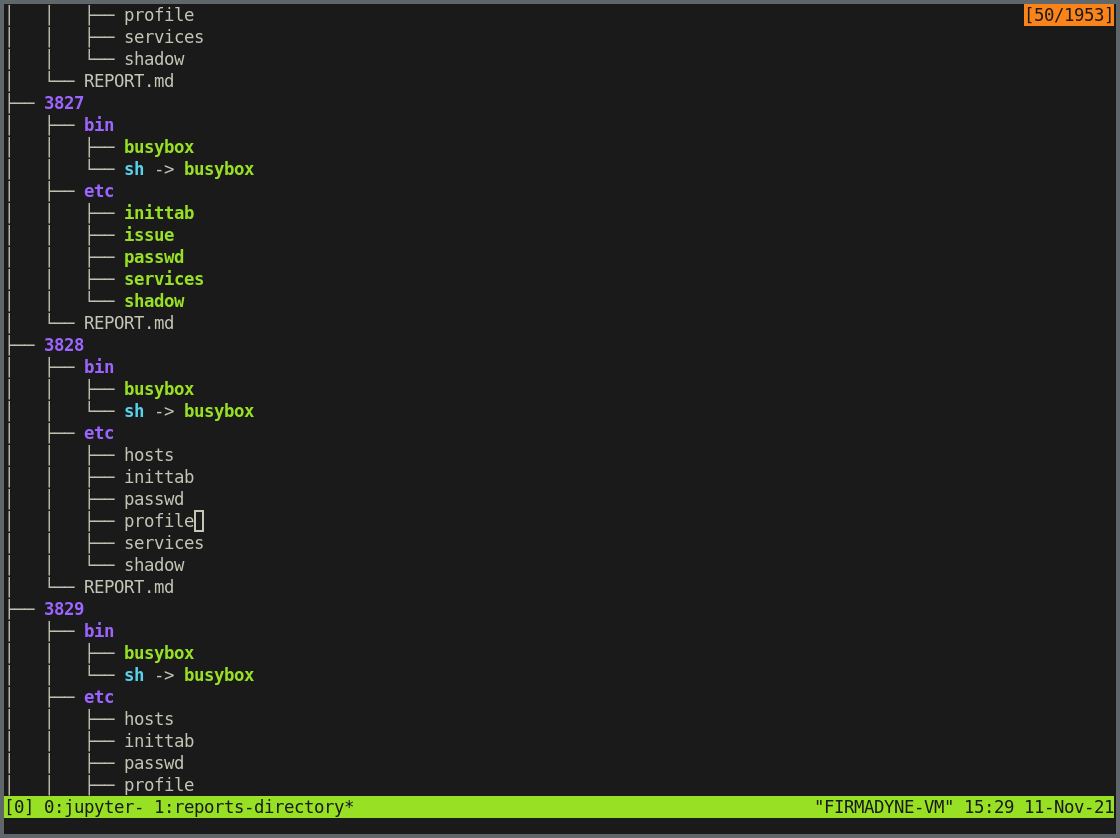
\includegraphics[width=0.65\textwidth]{figs/tree.png}
    \caption{Structure of the directory containing extracted firmware interesting files and the generated report for each firmware.}
    \label{fig:reports-directory}
\end{figure}

This structure was designed because at the same time that it is difficult to visually extract useful information from a large compilation of exposed firmware files together from a whole database of firmware images, it may be very useful for a security specialist to have separated the interesting files for a given firmware target. Sometimes just by looking at the content of an important configuration file, a professional can pinpoint a configuration that leads to a security breach. This way, if a professional wants to analyze the interesting files for a given firmware, he can easily browse the reports directory and search for the directory matching the ID of the target firmware.

More than that, this structure makes it easy to automatically generate pretty formatted reports of information for a given firmware target, and that is exactly what we implemented next.

Beyond automatically generating reports, saving the interesting firmware exposed files in a specific directory allows for batch processing and data mining in the whole dataset of exposed files for all extracted firmware exposed filesystems. This idea was not implemented in this work, but can be implemented in the future during the Clustering phase of the SCREEN project. The result of the mentioned analysis could find common hashes or common configuration files containing unsafe parameters.

\subsection{Automatically Generated Reports \& Exposed Files Samples}
\label{sec:auto-reports}

Using the code implemented in Section \ref{sec:firmware-content-statistics}, we then implemented a tool to automatically produce reports containing firmware information and interesting exposed files content for each firmware.

The reports were produced in raw text files using the Markdown language format. This way, a Markdown visualization software can be used to print the report in a beautiful processed way. In our repository \cite{github:c2dc-toso} we implemented a notebook to automatically produce the automatic reports for given firmware targets and also a notebook to visualize produced reports (after markdown compilation) for given target firmware targets.

Figure \ref{fig:automatic-report} shows the look of the first page of the report that was automatically produced for the firmware with ID = 11. If a security specialist wants to analyze the security of specific router firmware, the produced report can serve as a starting point to the specialist.

\begin{figure}[H]
    \centering
    \frame{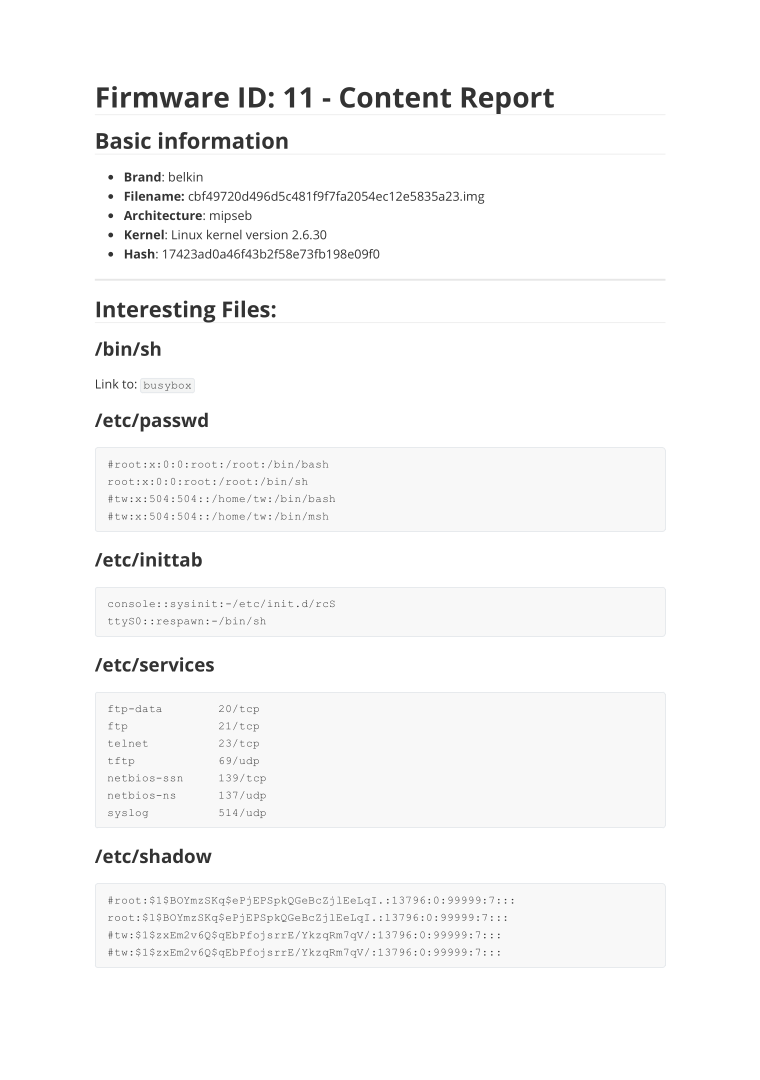
\includegraphics[width=0.75\textwidth]{figs/REPORT2.png}}
    \caption{The first page of a produced report in Markdown format for a given firmware target (in this case firmware with ID = 11).}
    \label{fig:automatic-report}
\end{figure}

Some examples of exposed interesting files we decided to include in the generated reports and the number of firmware images exposing these files are illustrated in Table \ref{tab:exposed-files}

\begin{table}[H]
\centering
\caption{Exposed interesting files found in firmware filesystems and included in the generated reports.}
\resizebox{\textwidth}{!}{\begin{tabular}{|c|c|c|}
\hline
\textbf{File}                           & \textbf{Description}                                                                   & \textbf{Number of files} \\ \hline

{\tt /etc/profile} or {\tt /profile}    & {\footnotesize System wide environment variable definitions.}                                                                                                    & 1505      \\

{\tt /etc/passwd} or {\tt /passwd}      & {\footnotesize \begin{tabular}[c]{@{}c@{}}File containing user login accounts (usernames),\\ default home directory and shell for each user.\end{tabular}}       & 1502      \\

{\tt /etc/inittab} or {\tt /inittab}    & {\footnotesize Init daemon configuration.}                                                                                                                       & 1057      \\ 

{\tt /etc/shadow} or {\tt /shadow}      & {\footnotesize Password hashes for system's account.}                                                                                                            & 912       \\

{\tt /etc/ssh/ssh\_host\_key}           & {\footnotesize \begin{tabular}[c]{@{}c@{}}Private SSH key\\({\color{red} \tt [Critical]} - Should not be exposed).\end{tabular}}                                            & 13        \\

{\tt /etc/ssh/sshd\_config} or {\tt /etc/sshd\_config} 
                                       & {\footnotesize SSH daemon configuration files.}                                                                                                                   & 6        \\ 

{\tt /etc/ssh/ssh\_config} or {\tt /etc/ssh\_config} 
                                       & {\footnotesize SSH client configuration files.}                                                                                                                   & 5        \\ \hline
\end{tabular}}
\label{tab:exposed-files}
\end{table}

Note that this exposed files search was simply conducted searching for specific files in common directories. If we implement a more advanced search (e.g search by file contents) we could possibly discover even more private SSH keys and credentials exposed in our firmware dataset.

Particularly the exposed private SSH keys are security-critical. Depending on how this SSH key is used by the products in question, if any device is configured to trust the public key associated with the exposed private SSH key, the content of the private key is enough to give an attacker free SSH access to a target.

An exposed SSH private key is enough to register a Common Vulnerabilities and Exposures (CVE) entry. The Common Vulnerabilities and Exposures is a system maintained by the United States government and by the not-for-profit Mitre Corporation in which publicly known information-security vulnerabilities and exposures are cataloged. When a new security vulnerability is discovered in software that has been publicly released, the person who discovered it can request to register a new entry in the database referring to the vulnerability discovery. The request is then curated, and if applicable the discovered vulnerability is registered and a unique identification number (usually called CVE number or CVE ID) is assigned to it. The CVE database can be publicly consulted\footnote{\url{https://www.cve.org/}}.

That being said, after consulting the CVE database for one of the firmware products with exposed SSH private keys, we discovered that the product (and vendor) is indeed listed on the database, but no CVE is registered for the product. Therefore, our team is eager to open a request to register the exposed private key vulnerabilities, as well as any other vulnerabilities we might discover during our ongoing research into the Common Vulnerabilities and Exposures system.

Continuing our examination, we also investigated what is the default shell used in the firmware images. As it is common for embedded devices, our intuition pointed that the default shell for the extracted firmware images would probably be the {\tt busybox} shell. Our investigation confirmed this intuition: From the 1279 identified shells for the extracted firmware, $96.60\%$ ($1208$) were {\tt busybox} shells and $5.40\%$ (69) were {\tt bash} shells, as shown in Table \ref{tab:shell-count}.

\begin{table}[H]
\centering
\caption{Identified shells in extracted firmware filesystems.}
\begin{tabular}{|c|c|}
\hline
\textbf{Shell} & \textbf{Number of Identified Shells} \\ \hline
{\tt busybox}        & 1208 (94.60\%)              \\
{\tt bash}           & 69 (5.40\%)                 \\ \hline
\end{tabular}
\label{tab:shell-count}
\end{table}

A recent post made by the cybersecurity team Claroty’s Team82 in partnership with JFrog (a company that develops leading solutions for DevOps and software updates management) claims that they made the discovery of 14 vulnerabilities inside the {\tt busybox} software. The registered CVE for each vulnerability suggests that these vulnerabilities allow for Denial of Service (DoS) and possible Remote Code Execution (RCE)~\cite{jfrog-busybox}. As shown by Table \ref{tab:shell-count}, the vulnerabilities in {\tt busybox} discovered by Claroty and JFrog are of great concern because most home wireless routers installed today may have vulnerable {\tt busybox} binaries and this could be another source for a large scale network attack. Because these vulnerabilities in {\tt busybox} were so recently disclosed, there was no able time to explore them. In future works, investigating the published CVE's for {\tt busybox} may be a great idea. More about future work suggestions in Section \ref{sec:future-work}.

\section{Kernel Cross-compilation \& Toolchain Building}

As shown by Table \ref{tab:kernel-family-stats}, kernel family 2.6 was the second most commonly found amongst successfully extracted kernels from commercial wireless router firmware and is a very old kernel family (the longest supported 2.6 kernel ended its life in 2016 although there is still one 2.6 kernel - 2.6.32 - that is still being maintained by Canonical Ltd.\footnote{\url{https://en.wikipedia.org/wiki/Linux_kernel_version_history}}). Therefore, we investigated the difficulties of cross-compiling a 2.6 Linux kernel. At first, we tried to cross-compile the kernel in a raw modern operating system. We chose Debian 10 (running with Linux kernel version 4.19) as the starting point for this experiment. In this environment, with {\tt gcc} version 8.3.0 as the compiler and using {\tt libc} version 2.28.10 it was not possible to compile the target kernel.

Then we downloaded an old version of the Debian operating system, with a release date similar to the 2.6 Linux kernel. Debian 3.1r8 (kernel 2.4.27) was used for this experiment. Using this old operating system, with {\tt gcc} version 3.3.5 as the compiler and using {\tt libc} version 2.3.2, we had success in compiling the target kernel.

% This highlights the impact the toolchain (compiler, binary utilities and library versions) has on kernel compiling process and therefore to achieve a way to automate kernel compiling, we also need a way to automate toolchain building. In this context, we adopted the {\tt crosstool-ng} tool. With this program, the user can define, between some pre-configured settings, specific versions for each tool inside the toolchain, and the program then tried to compile the desired toolchain.

This highlights the impact the toolchain (compiler, binary utilities and library versions) has on kernel compiling process and therefore to achieve a way to automate kernel compiling, we also need a way to automate toolchain building. In this context, we adopted a tool called {\tt crosstool-ng}\footnote{\url{https://github.com/crosstool-ng}}. The purpose of this tool is to help developers build their tools to other systems (especially for other architectures - a process called cross-compiling). To achieve that, {\tt crosstool-ng} allows the user to define, between some pre-configured settings, specific versions for each tool inside the toolchain used during software compile, and the program then tries to compile the desired toolchain. The user can then use the toolchain compiled by the {\tt crosstool-ng} to finally compile the desired software. Figure \ref{fig:crosstool} shows a diagram explaining the basic operation performed by the {\tt crosstool-ng}.

\begin{figure}[H]
    \centering
    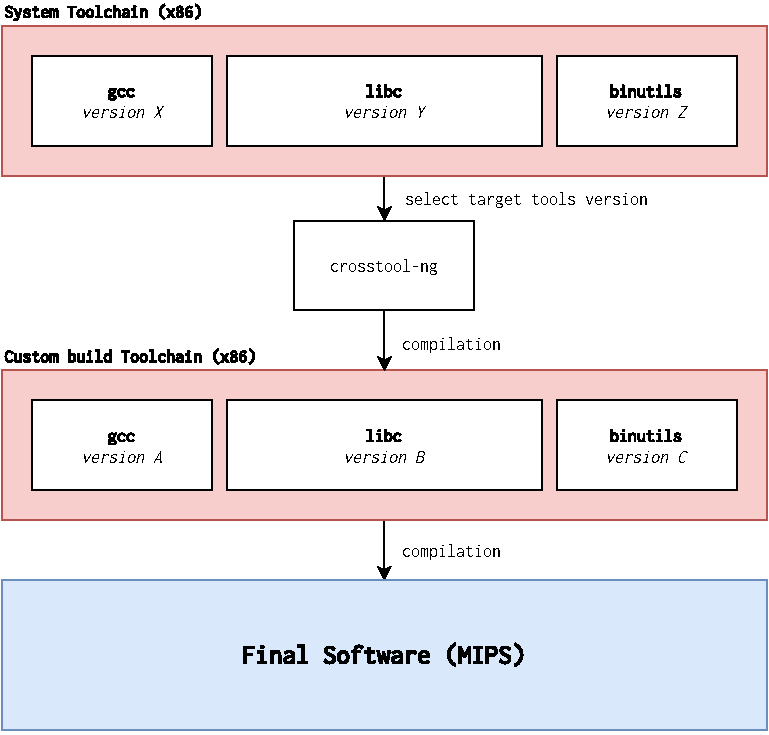
\includegraphics[width=0.65\textwidth]{figs/crosstool.pdf}
    \caption{Diagram illustrating the high-level view of the {\tt crosstool-ng} tool being used to compile software for the {\tt MIPS} architecture from a {\tt x86} host. Note that the system toolchain tools version is not the same as the custom build toolchain tools.}
    \label{fig:crosstool}
\end{figure}

Using {\tt crosstool-ng} we were then able to successfully compile a 2.6 Linux kernel inside a Debian 10 (modern operating system). However, when trying to cross-compile the target kernel for the {\tt MIPS} architecture (cross-compiling), we still faced issues that did not allow the kernel to compile successfully and further investigation is needed in order to build a working toolchain for this scenario. Nevertheless, {\tt crosstool-ng} seems to be an adequate tool to use in order to build an automated kernel compilation solution to support the SCREEN idealized architecture for re-hosting in the future.

\section{Firmware Re-hosting}

Regarding firmware re-hosting, in this section we will describe our team's efforts towards performing the re-hosting of the acquired wireless router firmware images to emulate its behavior with the intention to, in future work, analyze its overall security using an offensive security approach. We will describe our results obtained when taking both a more manual approach and a more automated one. The manual approach will follow a path that was already explored in the work of \cite{victor-sales} as a way to gain a minimum knowledge about the practical aspects involved in firmware re-hosting with QEMU. The automated approach will explore the Firmadyne~\cite{firmadyne} and Jetset~\cite{jetset} tools in order to perform re-hosting of firmware images in scale.

\subsection{Manual Re-hosting}
\label{sec:manual-rehosting}

Before evaluating the performance of automated tools in the process of re-hosting firmware, to better understand how the QEMU tool can be used to boot and emulate a system, we first investigated how to manually re-host a firmware configuring QEMU in system mode emulation and preparing a firmware image to be re-hosted. In its work, \cite{victor-sales} explains the fundamentals for manually re-hosting a downloaded firmware image and presents its results while emulating two different firmware images from wireless routers.

In \cite{victor-sales} work, re-hosting is done in a very similar approach with the one taken by Firmadyne~\cite{firmadyne} authors, in which firmware kernel is replaced with a pre-compiled similar Linux kernel, and then QEMU is used in system mode to boot the custom kernel. \cite{victor-sales} uses a pre-compiled Linux kernel version 2.6.35 with a minimal filesystem to boot a firmware and leverage QEMU network capabilities to bridge the host operating system and the system emulated with QEMU. After that, he uses the {\tt scp} utility (a command-line tool to copy files using the SSH protocol) to copy the contents of the original firmware filesystem to the re-hosted operating system running with QEMU.

We decided to follow the steps described for this ``manual'' firmware re-hosting to gain more understanding of the process. The firmware with ID = 11 was selected to be manually emulated (this was the first firmware id that showed up when querying the database). Before executing the steps to emulate the firmware with QEMU, reading the automatically generated report we implemented in Section \ref{sec:auto-reports} can already provide us with useful information about the firmware we want to re-host. Figure \ref{fig:automatic-report} already showed the first page of the report generated for the firmware with ID = 11 (our target firmware in this experiment). From the first page of the report we generated automatically we already have the pieces of information required for starting the manual re-hosting:

\begin{itemize}
    \item Firmware architecture is MIPS Big Endian ({\tt mipseb}): From the binaries provided by QEMU, we shall use the {\tt qemu-system-mips} executable to translate this firmware binaries correctly.
    \item Firmware original kernel is Linux kernel version 2.6.30.
    \item The {\tt /etc/inittab} file from this firmware is exposed and from its content we have the lead that the {\tt /etc/init.d/rcS} file from this firmware filesystem has the basics instructions of this router operation.
\end{itemize}

We then downloaded a basic Debian kernel version 2.6.32 (close to our target kernel version) and filesystem from a pre-compiled binary provided on the Debian project website\footnote{\url{https://people.debian.org/~aurel32/qemu/mips/}}. Following the instructions provided~\cite{victor-sales} the basic firmware boot consisted of executing the command shown in Code \ref{code:qemu-manual}.

\begin{listing}[!ht]
\inputminted[fontsize=\footnotesize,breaklines]{text}{Code/qemu-manual}
\caption{Command line to start QEMU in system mode running a minimal Debian running in MIPS architecture.}
\label{code:qemu-manual}
\end{listing}

This causes QEMU to open a window in which we can see the emulation of a screen connected to the firmware being re-hosted. As shown by Figure \ref{fig:qemu-manual}, the basic Debian kernel boots successfully using QEMU on system mode.

\begin{figure}[H]
     \centering
     \begin{subfigure}[b]{0.45\textwidth}
         \centering
         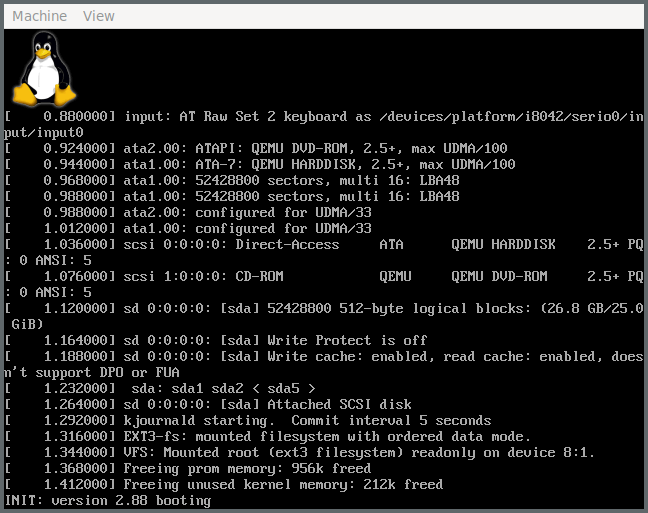
\includegraphics[width=\textwidth]{figs/qemu.png}
         \caption{Booting in process.}
         \label{fig:qemu-loading}
     \end{subfigure}
     \hfill
     \begin{subfigure}[b]{0.45\textwidth}
         \centering
         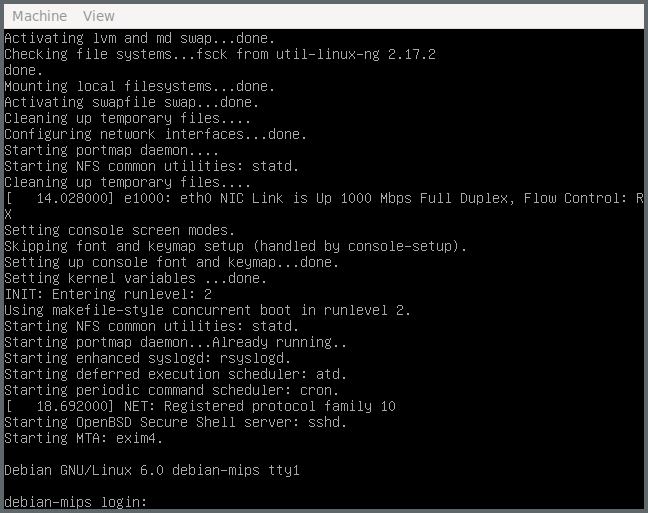
\includegraphics[width=\textwidth]{figs/qemu2.png}
         \caption{Boot completed.}
         \label{fig:qemu-booted}
     \end{subfigure}
        \caption{QEMU running on system mode emulating a Linux running on MIPS architecture.}
        \label{fig:qemu-manual}
\end{figure}

After the system has booted, we copied the original firmware filesystem contents into the emulated system using the {\tt scp} utility and rebooted the emulated system. After rebooting the firmware, with the original firmware contents in the filesystem, the boot process was not successful. This result was already expected based on what was reported by Sales~\cite{victor-sales} experiments.

\begin{figure}[H]
     \centering
     \begin{subfigure}[b]{0.45\textwidth}
         \centering
         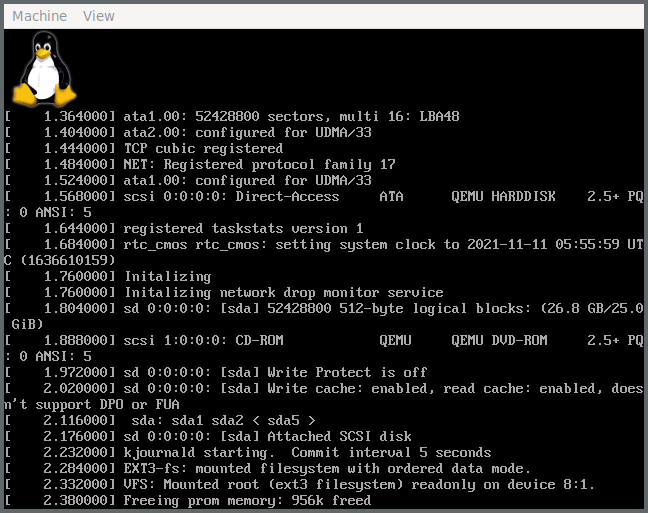
\includegraphics[width=\textwidth]{figs/qemu3.png}
         \caption{Booting in process.}
         \label{fig:qemu-loading}
     \end{subfigure}
     \hfill
     \begin{subfigure}[b]{0.45\textwidth}
         \centering
         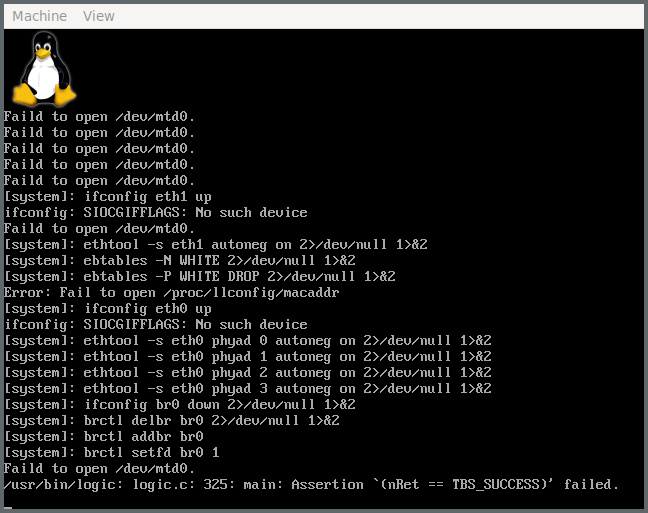
\includegraphics[width=\textwidth]{figs/qemu4.png}
         \caption{Failures during the boot process (Boot not completed).}
         \label{fig:qemu-booted}
     \end{subfigure}
        \caption{Failure in the booting process after overwriting the emulated filesystem with the original firmware filesystem.}
        \label{fig:qemu-manual-error}
\end{figure}

Next, we followed the approach of not copying all the files from the original firmware filesystem to the emulated machine, but only copying the most important files to emulate the firmware behavior. In this sense, we decided to read the {\tt /etc/inittab}, to discover the most prominent files loaded during the boot process (content shown in Figure \ref{fig:automatic-report}). The boot process ends after loading a file called {\tt /etc/init.d/rcS}. Inspecting the {\tt rcS} file contents, we discover that this file loads a lot of other files. Inspecting each of the loaded files, we discover that the {\tt /etc/init.d/daemon.rc} file finally loads the webserver behavior of the router. Code \ref{code:daemon.rc} shows the header of the {\tt /etc/init.d/daemon.rc} file.

\begin{listing}[!ht]
\inputminted[fontsize=\footnotesize]{bash}{Code/daemon.rc}
\caption{Header of the {\tt /etc/init.d/daemon.rc} file.}
\label{code:daemon.rc}
\end{listing}

This gives us an insight into this firmware's basic functionality. It uses the {\tt mini\_httpd} binary to host a Web Server and serves the {\tt /usr/www} directory. We were not successful when trying to execute the {\tt mini\_httpd} binary inside the emulated environment. It seems that the binary headers of the {\tt mini\_httpd} binary copied to the emulated machine had corrupted headers (error accused by the {\tt file} command inside the virtual system). As emulating firmware behavior individually is not the goal of our work, we ended the ``manual re-hosting'' here, as - although the firmware was not completely emulated - the experiment was already sufficient to provide valuable insights about the re-hosting process with QEMU and basic router firmware behavior.

Figure \ref{fig:illustrated-manual-rehosting} illustrates a diagram of the activities that were performed in order to execute this behavior emulation via manual re-hosting of the firmware.

\begin{figure}[H]
    \centering
    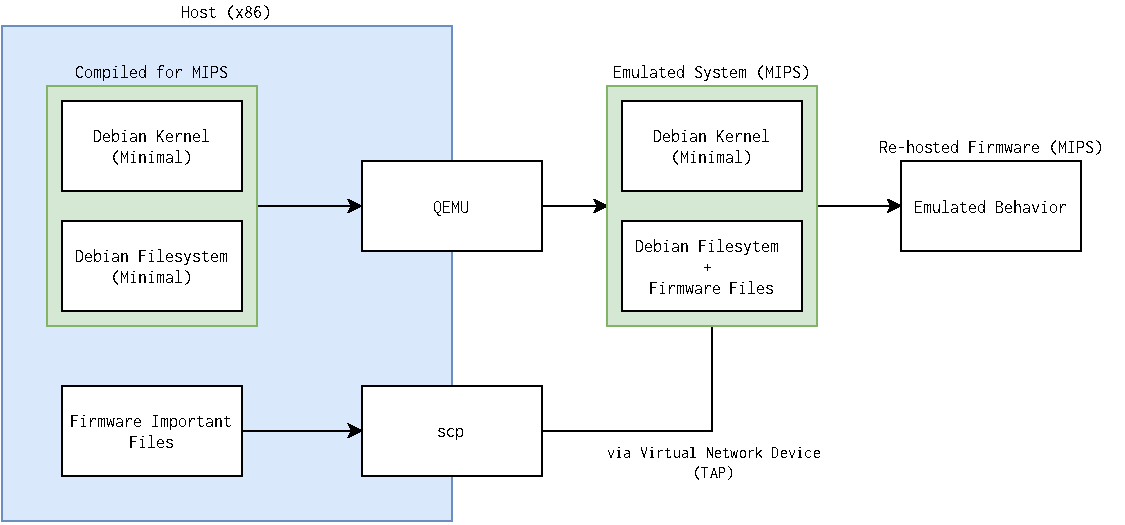
\includegraphics[width=0.9\textwidth]{figs/ManualReHosting.pdf}
    \caption{Diagram of the activities performed for manually emulating firmware behavior. Emulating a {\tt MIPS} firmware inside a {\tt x86} host machine. QEMU does the binary translation.}
    \label{fig:illustrated-manual-rehosting}
\end{figure}


\subsection{Re-hosting via Firmadyne}

Firmadyne provides scripts that can produce a {\tt QEMU} compatible disk from a firmware filesystem (that was previously extracted) applying some tweaks and patches in the filesystem of this produced disk. For instance, the script replaces the {\tt busybox} binary with a statically-compiled version, replaces the password of the root user for a default one, guarantees that the filesystem contains some critical files, replaces the Non-volatile random-access memory (NVRAM) library and many other minor tweaks.

This is already a great advantage when compared to the manual re-hosting described in Section \ref{sec:manual-rehosting}, because when manually copying the filesystem with the {\tt scp} utilities, we faced an error that prevented the firmware from successfully rebooting. Firmadyne implementation uses this approach of creating a system disk based on the original firmware filesystem and applying patches to fix the firmware boot (like the NVRAM patch). If a firmware boots successfully, its execution fidelity is considerably greater than the one we can have when emulating the firmware behavior simply by copying the most critical files served by the Hypertext Transfer Protocol (HTTP) server.

% ==========================================================================================================

The first experimentation with re-hosting via Firmadyne was to try to perform the re-hosting of at least one firmware by manually executing Firmadyne's instructions one by one. Selecting at random three firmware images that were successfully extracted and had the kernel version and architecture detected we made the first re-hosting experiments using the scripts provided by Firmadyne. The three selected firmware images on this steps were from the vendors Netgear, Belkin and Buffalo, executing Linux kernel version {\tt 3.14.4} ({\tt ARM}), {\tt 2.6.30} ({\tt MIPS}) and {\tt 3.10.1} ({\tt MIPS}) respectively.

While trying to re-host the selected firmware files with Firmadyne, only the Netgear firmware had its network interface successfully detected before the actual re-hosting. Table \ref{tab:fist-rehosting} shows the first results when trying to execute the Firmadyne's re-hosting capabilities for the three selected firmware images mentioned in the previous paragraph.

\begin{table}[H]
\centering
\caption{First results when experimenting with Re-hosting via Firmadyne. Firmware images selected at random. Minimal Firmadyne automation involved.}
\resizebox{\textwidth}{!}{\begin{tabular}{|c|c|c|c|c|c|}
\hline
\textbf{Firmware ID} & \textbf{Vendor} & \textbf{Architecture} & \textbf{Kernel} & \textbf{Network Interface} & \textbf{Result} \\ \hline
2                    & Netgear         & {\tt ARM}                   & {\tt 3.14.4}                  & {\tt 192.168.1.250}                       &  Missing Peripheral           \\
11                   & Belkin          & {\tt MIPS}                  & {\tt 2.6.30}                 & Not Detected                        &    Network Error                       \\
48                   & Buffalo         & {\tt MIPS}                 & {\tt 3.10.1}                 & Not Detected                        &        Kernel Panic                    \\ \hline
\end{tabular}}
\label{tab:fist-rehosting}
\end{table}

After blindly trying to execute Firmadyne's re-hosting capabilities and failing, we then tried to better understand the tool by extensively reading its code.  Analyzing Firmadyne's repository one can see that it does three basic steps in order to try the re-hosting of a well extracted and known firmware image (Firmadyne does not perform these steps automatically. The user has to execute them in order manually):

\begin{enumerate}
    \item For one extracted firmware filesystem, build a QEMU disk (emulates the disk image of a hard drive) applying the filesystem patches to bypass firmware peripherals dependencies. This process is costly and very slow because it requires uncompressing the firmware filesystem (saved in a directory inside our project), creating a virtual partition using {\tt fdisk}, and copying the extracted filesystem to this new partition, saving it to a file and storing it in a directory that is designed to hold these generated QEMU disks. This is done by the {\tt makeImage.sh} script from the Firmadyne repository.
    
    \item For an already built QEMU disk, Firmadyne then tries to infer which network Internet Protocol Address (IP Address) this router would probably use. This is done by starting a process similar to the final process of re-hosting. QEMU is started on system mode with the same exact command to be used in the next step to perform the final re-hosting of the firmware, but with a timeout of 60 seconds. During these 60 seconds the firmware is trying to boot with QEMU, Firmadyne then monitors the network interfaces of the host machine. When it detects changes in the host network, it associates this change with the firmware trying to boot within QEMU. This way Firmadyne tries to detect the interface address of the emulated firmware. When the network is detected, a customized run script specific for this firmware is saved in the image directory. The custom run script allows QEMU to launch the re-hosted firmware and also tells QEMU to create a network tunnel connecting with the network interface the re-hosted firmware is going to use. This allows us to ``reach'' the re-hosted firmware from our network. This is done by the {\tt inferNetwork.sh} script from the Firmadyne repository.
    
    \item Finally, the final step is to run the re-hosted firmware. This is done by simply executing the correct QEMU binary for a given architecture, and passing it as a parameter to the execution of QEMU: The pre-compiled and instrumented Linux kernel (has one version if running for a MIPS architecture and one version specific for ARM architecture), and the QEMU disk consisted of the target firmware filesystem with Firmadyne patches applied. This is done by the {\tt run.sh} script that is generated in the previous step (and not the one from the Firmadyne repository).
\end{enumerate}

After applying the {\tt inferNetwork.sh} script in a large number of firmware images (to generate the custom scripts in batch), we received a lot of negative results (interfaces not being detected). Debugging what could be the cause, we discovered that the default {\tt run.sh} script that is used to try to boot the firmware in this step of network detection, redirects the output of the firmware to a file in the hard drive. This process really slows down firmware execution, in the sense that the 60 seconds timeout defined for the network detection phase is not enough. We changed the scripts to use a directory that was mounted in the TMPFS, hoping that redirecting the output to the RAM could increase the emulation speed. It worked, and after running the {\tt inferNetwork.sh} again we finally could see more firmware having its network interface detected. Because of the 60 seconds timeout, and because only one {\tt inferNetwork.sh} can run at a time (because a network address collision happens when trying to run more than once), this process is also slow and not very effective, as it takes at least 60 seconds per firmware vendor and it requires to be executed in a sequential way.

\textbf{COLOCAR UMA ESTATÍSTICA (TABELA) AQUI}


After executing the network inference, we tried then executing the generated {\tt run.sh} for some of the firmware with the correctly identified network interface. When executing Firmadyne~\cite{firmadyne} with the sample firmware provided by the repository (downloaded from a vendor website), the re-hosting phase of the firmware emulation is indeed successful, as illustrated by Figure \ref{fig:emulated-sucess}.

\begin{figure}[H]
     \centering
     \begin{subfigure}[b]{0.45\textwidth}
         \centering
         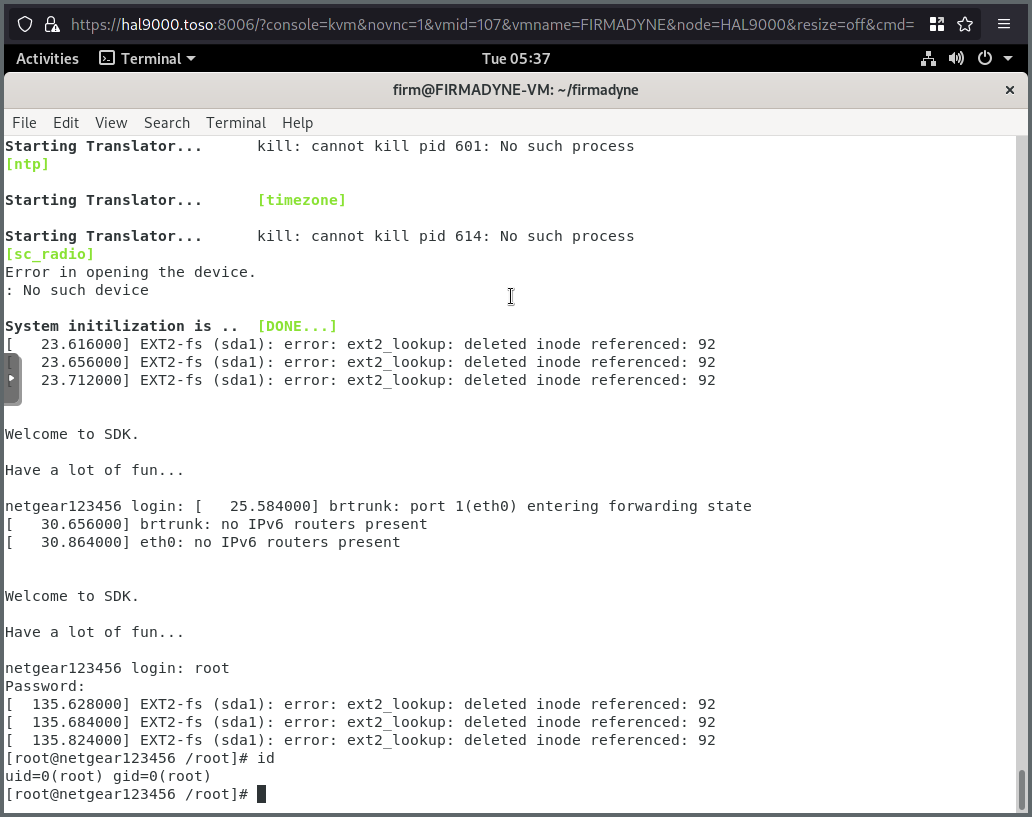
\includegraphics[width=\textwidth]{figs/sucess.png}
         \caption{Re-hosted firmware booted successfully.}
         \label{fig:qemu-sucess1}
     \end{subfigure}
     \hfill
     \begin{subfigure}[b]{0.45\textwidth}
         \centering
         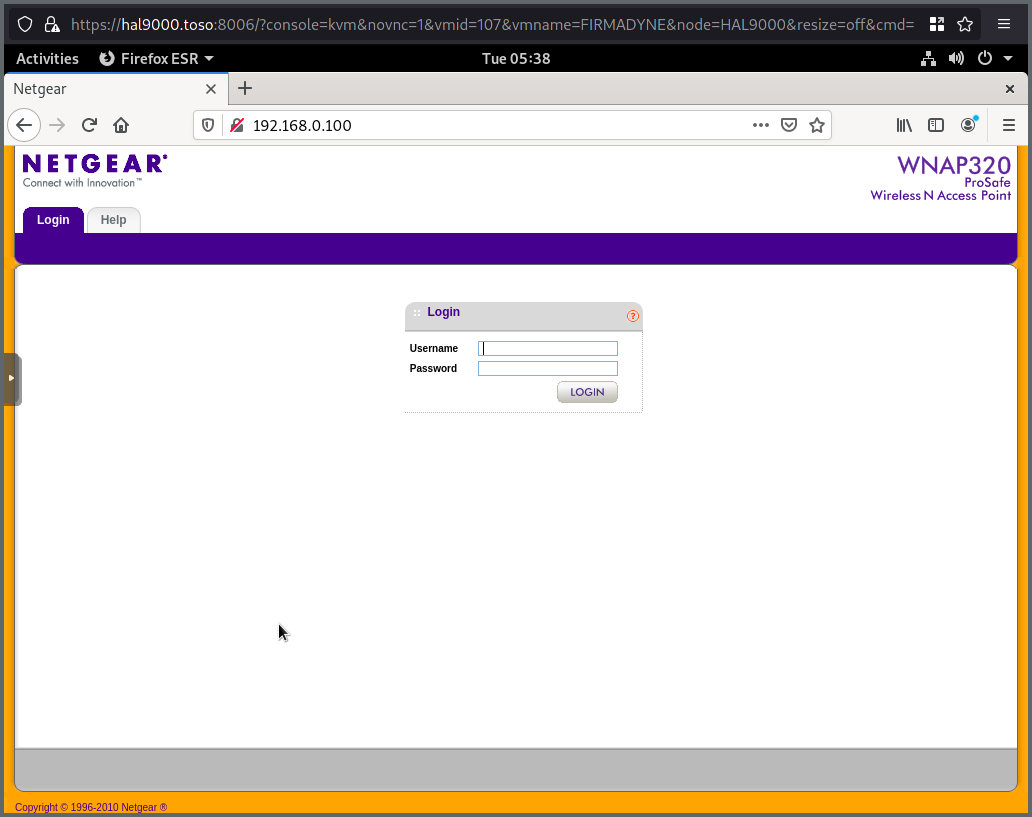
\includegraphics[width=\textwidth]{figs/sucess2.png}
     The w    \caption{Web interface of the re-hosted firmware.}
         \label{fig:qemu-sucess2}
     \end{subfigure}
        \caption{Firmadyne successfully re-hosting the sample firmware. Firmware designed to run on {\tt ARM} running on {\tt x86}.}
        \label{fig:emulated-sucess}
\end{figure}

However, when executing with the firmware images in our dataset (acquired by the scraper and enumerated by the process described in the previous sections), the results are still very diverse. A lot of different errors appear when trying to emulate some firmware images, for instance complaints about not found NVRAM entry keys (Firmadyne allows for compiling a new {\tt libnvram} containing custom used added keys) or errors when the firmware execution is trying to access a peripheral that is not found by the system (for instance in our case we see many firmware executions complaining when trying to access files that would be related to a display LED). Figure \ref{fig:firmadyne-errors} shows some of the different error messages we obtained for different firmware images during re-hosting. But we also could indeed re-host some of the firmware with success, as shown by Figure \ref{fig:firmadyne-success} in which it is shown the post-boot login console from a firmware designed to execute on the {\tt MIPS} architecture running on our {\tt x86} computer.

\begin{figure}[H]
     \centering
     \begin{subfigure}[b]{0.45\textwidth}
         \centering
         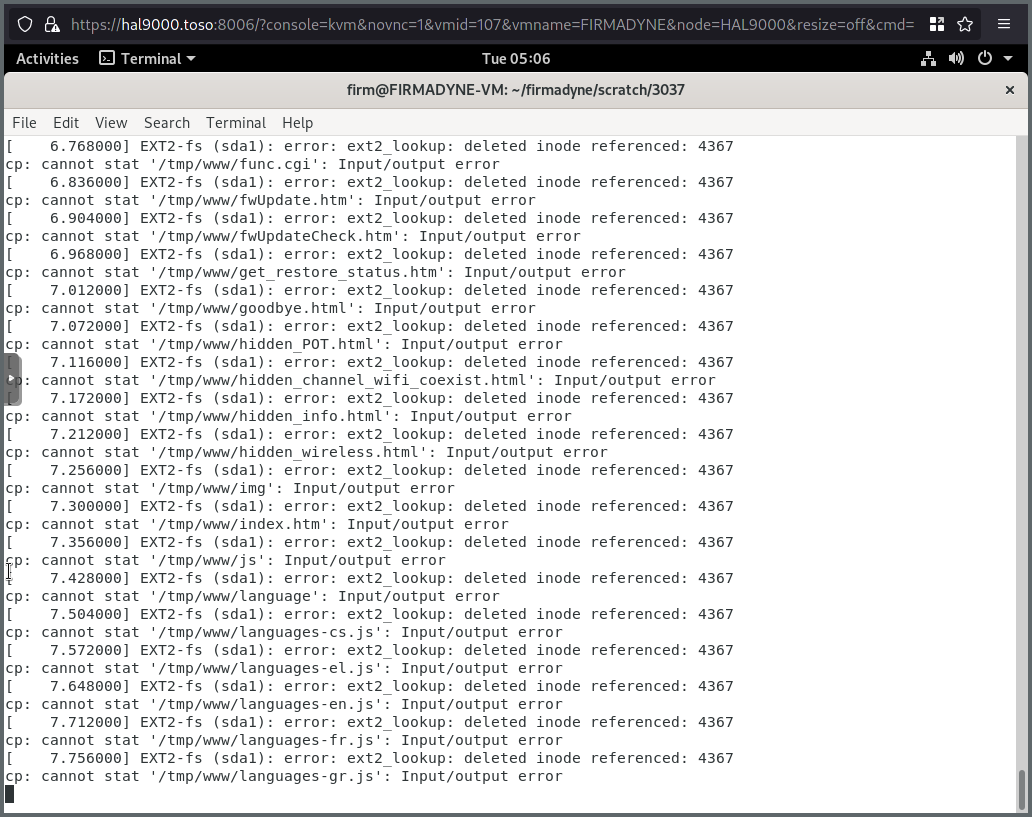
\includegraphics[width=\textwidth]{figs/ext2-error.png}
         \caption{Error trying to access files.}
         \label{fig:}
     \end{subfigure}
     \hfill
     \begin{subfigure}[b]{0.45\textwidth}
         \centering
         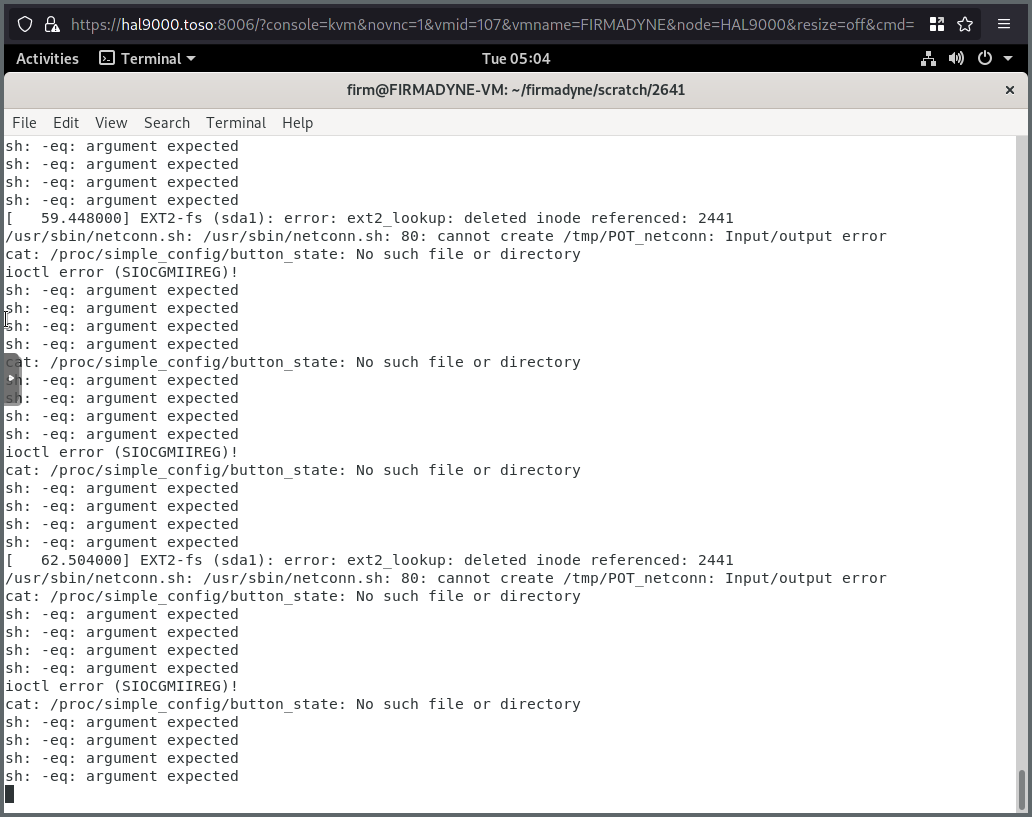
\includegraphics[width=\textwidth]{figs/ioctl2-error.png}
         \caption{{\tt ioctl} error and missing peripheral.}
         \label{fig:}
     \end{subfigure}
     \hfill
     \begin{subfigure}[b]{0.45\textwidth}
         \centering
         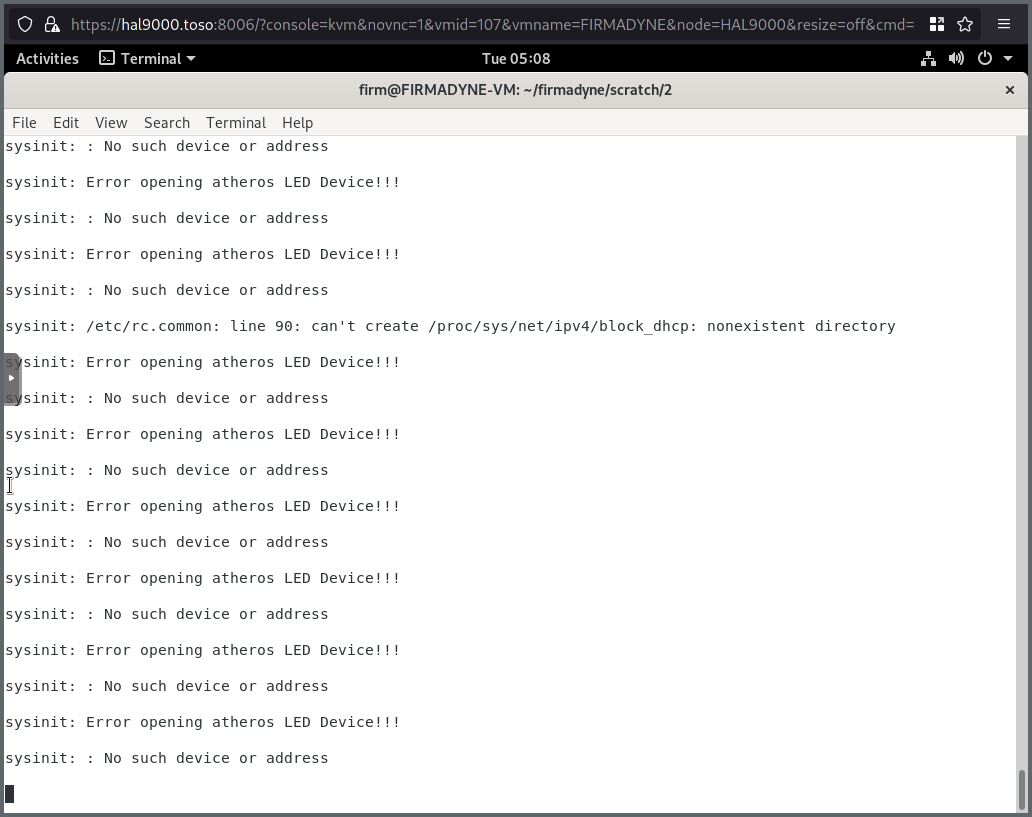
\includegraphics[width=\textwidth]{figs/led-error.png}
         \caption{{\tt sysinit} error because of missing peripheral.}
         \label{fig:}
     \end{subfigure}
     \hfill
     \begin{subfigure}[b]{0.45\textwidth}
         \centering
         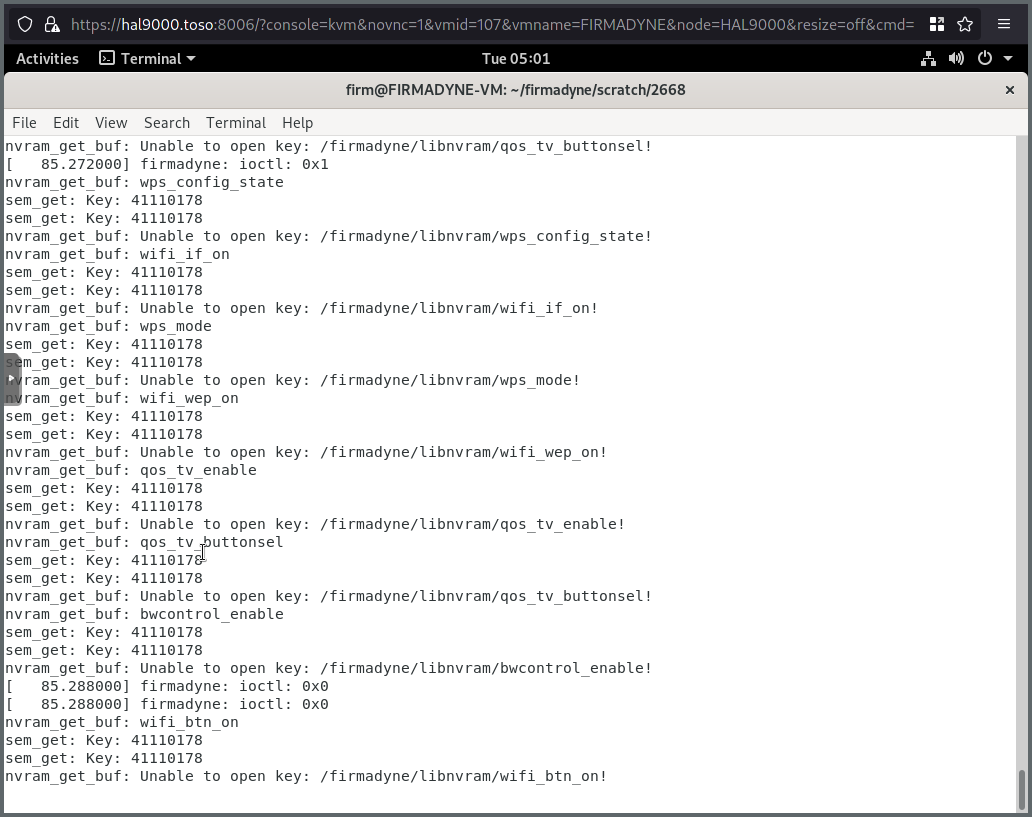
\includegraphics[width=\textwidth]{figs/nvram-error.png}
         \caption{Missing NVRAM key error.}
         \label{fig:}
     \end{subfigure}
        \caption{Errors faced when trying to re-host different firmware images from our dataset.}
        \label{fig:firmadyne-errors}
\end{figure}

\begin{figure}[H]
    \centering
    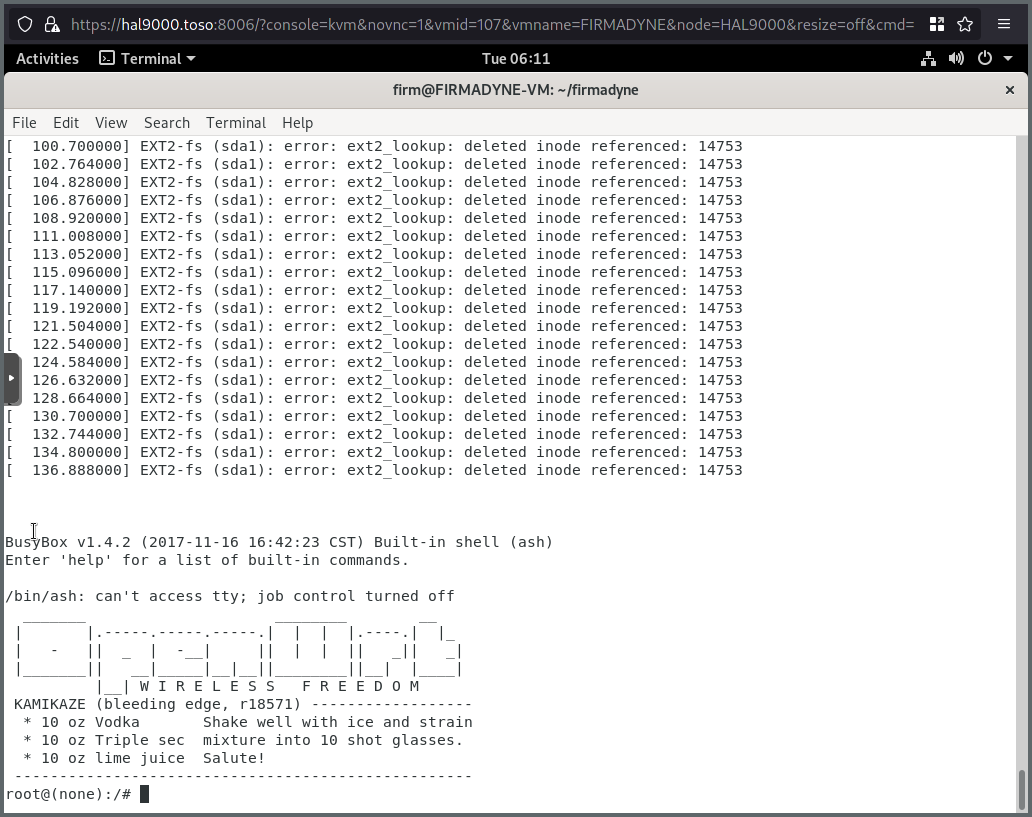
\includegraphics[width=0.85\textwidth]{figs/firmadyne-success.png}
    \caption{Firmadyne successfully re-hosting the sample fimrware. Firmware designed to run on {\tt MIPS} running on {\tt x86}.}
    \label{fig:firmadyne-success}
\end{figure}

The results obtained when executing the final re-hosting steps with Firmadyne are very diverse. We can perceive that the idea used does work, as we have firmware that can successfully boot and work as intended. However, there are still lots of errors present on the boot process of most of the images. Most of the errors are related to missing entries on the NVRAM or missing files. Adding more entries and recompiling the {\tt libnvram} may help with the missing entries; enhancing the extraction process we may find that the firmware contains more than one partition, and thus, we could seek the missing files. Moreover, one difficult task is on how to evaluate in scale if the booting process was successfully or not. For an individual firmware image, a human can easily tell when the firmware was able to boot without problems. But finding a way to check this at scale is still something to debate. Firmadyne uses a mere {\tt ping} to check if the firmware is available on the local network. If the firmware answers the network packet then it considers that the firmware had it's boot successful. Although this already brings some automation to the table, it is still not the ideal solution.


\subsection{Re-hosting via Jetset}
\label{sec:result-jetset}

Jetset~\cite{jetset} uses a symbolic execution engine with a custom developed algorithm to try to boot a firmware from a device with peripherals dependencies, as already discussed in Chapter \ref{chap:related}. We believe this novel approach is very clever, and we want to investigate further to discover if it could fit our project. However, to the scope and time range of this paper, we only read it's source code to understand the tool principles and tested Jetset with it's default proof-of-concept firmware images that were used to produce it's article (and so we had at hand all the necessary inputs to start the firmware symbolic inference).

In future works (see Section \ref{sec:future-work}) we intend to deeper understand the tool (we are going to need to gain more knowledge about symbolic execution as well) and try to integrate it into our SCREEN project if we can prove it is going to be of help in the task of re-hosting wireless router firmware devices.

% Virou parte da conclusão
% \chapter{Future Work}\label{chap:future-work}
% The work described in this document is part of an ongoing research project and its purpose is mostly to describe the approach we intend to use during the research. That being said, the main research and implementation is yet to happen next semester. The following section presents the next planned steps and schedule for this research work:

\section{Activities Schedule}

\begin{enumerate}
    \item Finish work environment setup and firmware acquisition process.
    \begin{itemize}
        \item Expect to finish until the end of \textbf{June, 2021};
    \end{itemize}

    \item Enhance firmware extraction process.
    \begin{itemize}
        \item Expect to finish until mid \textbf{July, 2021};
    \end{itemize}
    
    \item Setting up a toolchain building for kernel cross-compilation.
    \begin{itemize}
        \item Expect to finish until the end of \textbf{July, 2021};
    \end{itemize}
    
    \item Re-host firmware images using the compiled kernels and fix incompatibilities
    \begin{itemize}
        \item Expect to finish until mid \textbf{September, 2021};
    \end{itemize}
    
    \item Enhance the re-hosting process and evaluate the emulated firmware performance regarding its network capabilities \& Execute vulnerability discovery techniques in the emulated systems.
    \begin{itemize}
        \item Expect to finish until the end of \textbf{October, 2021};
    \end{itemize}
    
    \item Final paper adjustments and conclusion
    \begin{itemize}
        \item Expect to finish until \textbf{November, 2021};
    \end{itemize}
\end{enumerate}

\chapter{Conclusions, Contributions and Future Works}\label{chap:conclusions}
TODO (WIP)

Anotações:
\begin{itemize}

    \item Uma contribuição é o recoinassance de firmwares de roteadores
    \item Portanto permite explorar falhas como a do busybox
    \item Explorar as chaves privadas expostas (pelo vendor D-Link)
    \item Potencial fonte de CVE
    \item Re-hosting de kernel é um problema em aberto
    
\end{itemize}

\section{Contributions}

\subsection{Firmware Enumeration Statistics \& Reports}
One of the contributions of this work is that it provides insightful statistics about the software components and hardware architecture running on wireless router firmware. These statistics are not publicly available information and more than the actual numbers, this work produces a way to produce these statistics (that will become even more accurate if updating the scraper). Moreover, we implemented a tool to easily extract target files from multiple compressed filesystems at once, and to produce automated reports that can help the security specialist when working with individual firmware.

\subsection{Paper published in congress proceedings}
During the first experiments described in this paper we wrote an article~\cite{sbseg2021} that was approved for the XV Workshop on Scientific Initiation and Undergraduate Works (WTICG), an event that is part of the Brazilian Symposium on Information Security and Computer Systems (SBSeg). The article was published in SBSeg 2021 proceedings and can be checked online in the event web page\footnote{\url{https://sol.sbc.org.br/index.php/sbseg_estendido/article/view/17351}}. However, it is important to highlight here that the firmware dataset we used for the SBSeg 2021 paper was different for the one used in this work. A technical problem in our first machine forced us to download a new firmware dataset. Both fimrware images dataset were acquired the same way (using the scraper), but this work uses more spiders to acquire firmware images from a more diverse range of vendors (all vendors implemented by the scraper).

\subsection{GitHub Repository}
Code developed to support this work and jupyter notebooks containing code to extract data and perform re-hosting experiments (and the produced output) are available online in our GitHub repository~\cite{github:c2dc-toso}. People can feel free to copy our code to reproduce our analysis. As the work described in this paper is part of an ongoing research project, the repository will be kept being updated while for at least while the project is ongoing. We also welcome every kind of external contributions to our repository and work, be it code contributions, documentation or even mere code or research suggestions. Our GitHub repository named {\tt screen-toso} can be found online on GitHub\footnote{\url{https://github.com/c2dc/screen-toso}}.

\section{Future Work}
\label{sec:future-work}

The work described in this document is part of an ongoing research project that is being conducted with a group of researchers. Collaborating with our research we have academics and professionals from the military and the industry. This paper discussed only the first steps in experimenting with firmware analysis and re-hosting. As we gain more knowledge and develop our capabilities, more the SCREEN architecture described in Chapter \ref{chap:screen} can become a concrete product. It is even important to note that this present researcher is going to directly continue the work described in the paper as a Graduate research (that is already ongoing as part of the PMG - Masters in Graduation Program - offered by the Aeronautics Institute of Technology).

That being said, we have already envisioned a lot of ideas that can lead to future work and research extensions. Below we present some of the ideas proposed for future works:

\begin{itemize}
    \item \textit{Continue to investigate firmware Re-hosting solutions:} This is the most important task in which we will certainly keep working. Firmware re-hosting is still an open problem. Every solution we researched proposes a novel approach to re-hosting that offers different trade-offs in the emulation fidelity. Applying the proposed techniques in our real firmware images dataset is challenging as, although usually open source, most work published on firmware re-hosting had it's code implemented with research purposes in mind and therefore it usually does not contain extensive documentation and is not as easy to comprehend and extend nor robust as a commercial open source project.
    
    Still, experimenting with the implemented research solutions to re-hosting is very important to understand the already explored approaches on re-hosting. From this line of work, one can also combine complementary approaches and code to enhance the state of the art on firmware re-hosting. For instance, the automation implemented by Firmadyne~\cite{firmadyne} could be prepared to work together with the symbolic execution idea behind Jetset~\cite{jetset}. To achieve this, one of course may have to solve the problem of escalating the acquisition of the information needed as input for Jetset, that is related to the System-on-Chip (SoC) of the hardware being emulated and also update Firmadyne's database to store the relevant data.
    
    Another, even simpler open task for future work is to extend the idea of a patched kernel and filesystem that Firmadyne uses before trying to re-host a firmware to the automation we propose for kernel compile so that the patches are applied during kernel automated compile.
    
    \item \textit{Enhance the extraction process:} Firmware extraction process is based on an old Binwalk API and code can be updated to better use the Binwalk tool. Furthermore, the extraction process is very slow, some firmware images extraction hangs and the extractor has issues when working in parallel mode. Therefore the extraction phase can receive a lot of contributions. Also, visual inspection of the firmware images that were not correctly extracted by the extraction script can provide insights that can extend the number of firmware images we are able to extract (as it happened with the incorrect MIME type detection mentioned in Section \ref{sec:firmware-extraction}).
    
    \item \textit{Development of a automated firmware analysis product:} As we gained a lot of knowledge about firmware analysis during this work and because we already developed tools to automatically detect relevant content inside a firmware to automatically generate reports, this idea could be extended and a product could be developed to serve as an entry point to a security researcher when doing targeted firmware analysis. To achieve this we could increase the number of relevant files we search inside a firmware and also enhance to search firmware files from it's content in order to produce the reports to the analyst. The tool could also implement the simplest re-hosting techniques of the target firmware, and allow the security researcher using the tool to edit the QEMU parameters as intended.
    
    Also, even when working in scale as it's our original goal, there is a lot of ways as a product can be developed to make use of the already implemented tools and in the same time provide utilities to the operator. For instance a graphical tool to interact with the great amount of firmware images and to explore the databases and reports would already be handy. Our Jupyter notebooks and database SQL queries were already a primitive way to ease the interaction with the large amount of files, but one could benefit a lot from having a even more interactive and visual tool.
    
    \item \textit{Explore the {\tt busybox} disclosed vulnerabilities:} As mentioned in Section \ref{sec:auto-reports}, a computer security research team claims to have discovered new security breaches in the {\tt busybox} software. As {\tt busybox} represents 94.60\% of the identified shells used by the enumerated firmware, exploring the new vulnerability discovered for this product may lead to a new attack approach.
    
    \item \textit{Search for more exposed private SSH keys and request a CVE registration for the ones we found:} In Section \ref{sec:auto-reports} we mention that a CVE can be requested to register the exposed private SSH key for the 13 enumerated firmware images that have this issue. To register this exposure into the CVE system is already a task we are working on. Moreover, implementing a new mechanism to search firmware filesystem files by their contents can lead to more exposed private keys inside firmware files and is another idea of future work for this project.
    
    \item \textit{Investigate Jetset and other state-of-art tools:} As already mentioned in Section \ref{sec:result-jetset}, Jetset~\cite{jetset} seems to be a novel approach that can be of help to our task. The work however is very new and we could not test if deeper in a timely manner. For our future works we want to investigate if the Jetset can be added to our architecture and maybe integrate it with the Firmadyne re-hosting approach. To test other state-of-art tools product of other recent articles and published work may also be insightful and could help our research.
\end{itemize}

% \chapter{Introdução}
% \input{Capitulos/cap1}

% \chapter{Trabalhos Anteriores}\label{cap:past-works}
% \input{Capitulos/cap2}

% \chapter{Proposta}\label{cap:proposal}
% \input{Capitulos/cap3}


% REFERENCIAS BIBLIOGRAFICAS
\renewcommand\bibname{\itareferencesnamebabel} %renomear título do capítulo referências
\bibliography{referencias}

% \annex
% \chapter{Exemplo em WSDL}\label{anex:wsdl-example}
% \begin{minted}{xml}
<?xml version="1.0" encoding="UTF-8"?>
<description xmlns="http://www.w3.org/ns/wsdl"
             xmlns:tns="http://www.tmsws.com/wsdl20sample"
             xmlns:whttp="http://schemas.xmlsoap.org/wsdl/http/"
             xmlns:wsoap="http://schemas.xmlsoap.org/wsdl/soap/"
             targetNamespace="http://www.tmsws.com/wsdl20sample">

<documentation>
  This is a sample WSDL 2.0 document.
</documentation>

<!-- Abstract type -->
  <types>
    <xs:schema xmlns:xs="http://www.w3.org/2001/XMLSchema"
               xmlns="http://www.tmsws.com/wsdl20sample"
               targetNamespace="http://www.example.com/wsdl20sample">

     <xs:element name="request"> ... </xs:element>
     <xs:element name="response"> ... </xs:element>
    </xs:schema>
  </types>

<!-- Abstract interfaces -->
  <interface name="Interface1">
    <fault name="Error1" element="tns:response"/>
    <operation name="Get" pattern="http://www.w3.org/ns/wsdl/in-out">
      <input messageLabel="In" element="tns:request"/>
      <output messageLabel="Out" element="tns:response"/>
    </operation>
  </interface>

<!-- Concrete Binding Over HTTP -->
  <binding name="HttpBinding" interface="tns:Interface1"
           type="http://www.w3.org/ns/wsdl/http">
    <operation ref="tns:Get" whttp:method="GET"/>
  </binding>

<!-- Concrete Binding with SOAP-->
  <binding name="SoapBinding" interface="tns:Interface1"
           type="http://www.w3.org/ns/wsdl/soap"
           wsoap:protocol="http://www.w3.org/2003/05/soap/bindings/HTTP/"
           wsoap:mepDefault="http://www.w3.org/2003/05/soap/mep/request-response">
    <operation ref="tns:Get" />
  </binding>

<!-- Web Service offering endpoints for both bindings-->
  <service name="Service1" interface="tns:Interface1">
    <endpoint name="HttpEndpoint"
              binding="tns:HttpBinding"
              address="http://www.example.com/rest/"/>
    <endpoint name="SoapEndpoint"
              binding="tns:SoapBinding"
              address="http://www.example.com/soap/"/>
  </service>
</description>
\end{minted}


% \chapter{Exemplo em OpenAPI}\label{anex:openapi-example}
% \input{Anexos/anexoB.tex}

% \chapter{Exemplo em Protocol Buffers}\label{anex:protobuf-example}
% \input{Anexos/anexoC.tex}

% Glossario
%\itaglossary
%\printglossary

% Folha de Registro do Documento
% Valores dos campos do formulario

% [ ] - PREENCHER ISSO DIREITO ANTES DE ENVIAR PARA A BIBLIOTECA
\FRDitadata{XX de novembro de 2021}
\FRDitadocnro{DCTA/ITA/TC-056/2021} %(o número de registro você solicita a biblioteca)
\FRDitaorgaointerno{Instituto Tecnológico de Aeronáutica -- ITA}
%Exemplo no caso de pós-graduação: Instituto Tecnol{\'o}gico de Aeron{\'a}utica -- ITA
\FRDitapalavrasautor{Firmware; Security; Cybersecurity; IoT; Embedded; Linux; Re-hosting; MIPS; ARM; Emulation.}
\FRDitapalavrasresult{Sistemas de computadores embarcados; Cibernética; Segurança de Computadores; Avaliação de ameaças; Computação}
%Exemplo no caso de graduação (TG):
%\FRDitapalavraapresentacao{Final Paper, ITA, São José dos Campos, 2021. \NumPenultimaPagina\ páginas.}
\FRDitapalavraapresentacao{ITA, São José dos Campos. Curso de Graduação em Engenharia de Computação. Orientador: Prof. Dr. Lourenço Alves Pereira Jr. Publicado em 2021.}
%Exemplo no caso de pós-graduação (msc, dsc):
%\FRDitapalavraapresentacao{ITA, São José dos Campos. Curso de Mestrado. Programa de Pós-Graduação em Engenharia Aeronáutica e Mecânica. Área de Sistemas Aeroespaciais e Mecatrônica. Orientador: Prof.~Dr. Adalberto Santos Dupont. Coorientadora: Prof$^\textnormal{a}$.~Dr$^\textnormal{a}$. Doralice Serra. Defesa em 05/03/2015. Publicada em 25/03/2015.}
%\FRDitaresumo{% The widespread adoption of the home office weakens corporate networks, as it extends its perimeter to homes and ineffective security policies designed for different operating environments. In this context, wireless network routers serve as enablers of access to critical services. This is why studying embedded devices' software security is important to help vendors identify software flaws that lead to security vulnerabilities so they can fix them and enhance the security of their devices. This way, a large-scale cybersecurity attack leveraging insecure IoT devices can be avoided. However, identifying the software artifacts and possible vulnerabilities present on these devices is challenging. 

% One approach for inspecting the security of embedded firmware is to use system emulation to re-host the firmware execution to another machine from which security analysis can be performed. Nonetheless, firmware re-hosting is an open problem, motivating a lot of popular research on new techniques and approaches. This work aims to explore wireless router firmware security by enumerating its content to leverage information and statistics that enhance the performance of state-of-the-art re-hosting solutions for firmware analysis.

% To achieve this, we present our efforts in the analysis of $9176$ firmware images downloaded from $11$ vendors' sites and $3$ open-source firmware projects, yielding statistics of the most common operating systems and services present on these devices and automatically generating reports containing the most relevant information and important exposed files found on each firmware. Afterward, we present our results when trying to apply state-of-the-art solutions of re-hosting to some of our acquired firmware images.

A adoção em larga escala do trabalho remoto enfraquece as redes corporativas, visto que o perímetro desses redes é expandido para incluir domicílios e políticas ineficazes de segurança. Nesse contexto, roteadores de redes sem-fio servem como possibilitadores de acesso para serviços críticos. Por isso mesmo, estudar a segurança de \textit{software} de dispositivos embarcados é importante para auxiliar fabricantes a encontrar falhas de \textit{software} que causem vulnerabilidades de segurança, para estes consigam aplicar as devidas correções e aumentar a defesa de seus dispositivos.
Nesse sentido, pode-se evitar a ocorrencia de um ataque cibernético em larga-escala que se aproveite de dispositivos \textit{IoT} inseguros. No entanto, identificar os artefatos de \textit{software} e possíveis vulnerabilidades de segurança presente nesses dispositivos é desafiador.

%Nesse sentido, um ataque cibernético em larga-escala se aproveitando de dispositivos de \textit{IoT} inseguros pode ser evitado. 

Uma abordagem para a inspeção de segurança de \textit{firmwares} embarcados é utilizar a emulação ao nível de sistema para realizar a execução do \textit{firmware} em outra máquina a partir da qual análises de segurança possam ser realizadas. No entanto, o \textit{re-hosting} de \textit{firmwares} é um problema é aberto, e motiva diversas pesquisas recentes sobre novas técnicas e abordagens. Este trabalho visa explorar a segurança de \textit{firmwares} de roteadores sem-fio através da enumeração de seu conteúdo para o levantamento de informações e estatísticas que melhorem o desempenho das soluções estado-da-arte para a análise de segurança de \textit{firmwares} via \textit{re-hosting}.

Para isso, serão apresentados os esforços realizados para a análise de 9176 arquivos de \textit{firmware} obtidos dos \textit{websites} de 11 fabricantes e 3 projetos de \textit{firmware} de código-aberto, produzindo estatísticas dos serviços e sistemas operacionais mais presentes nesses dispositivos, além da geração automática de relatórios contento as informações mais relevantes e arquivos expostos encontrados em cada \textit{firmware}. Posteriormente, serão também apresentados os resultados obtidos a partir da aplicação das ferramentas estado-da-arte para a execução de \textit{re-hosting}, nos arquivos de \textit{firmware} obtidos.}
\FRDitaresumo{TODO

% OLD ABSTRACT, NEED TO DO A NEW ONE AFTER THE WORK IS DONE

% Studying embedded devices software security is important to help vendors identify software flaws that lead to security vulnerabilities so they can fix them and enhance their devices security. This way, a cybersecurity attack leveraging insecure IoT devices can be avoided. In this preliminary work we describe a way to automate security analysis on wireless routers firmware. Our proposal is to automatically acquire firmware images from vendor websites, extract kernel and filesystem from the acquired images and then re-host the firmware inside an emulator to use known techniques of vulnerability discovery.

}
%  Primeiro Parametro: Nacional ou Internacional -- N/I
%  Segundo parametro: Ostensivo, Reservado, Confidencial ou Secreto -- O/R/C/S
\FRDitaOpcoes{N}{O}
% Cria o formulario
\itaFRD


\end{document}

% Fim do Documento. O massacre acabou!!! :-)
